\chapter{Hardware description}
MANDEYE DEV is composed of (figure \ref{fig:m1}):
\begin{itemize}
	\item MANDEYE DEV main unit,
	\item Tool for nuts,
	\item Charger.
\end{itemize}
It is stored in suitcase for secure transport (figure \ref{fig:m2}).

\section{Turn on device}
Please click button on the bottom of the RONIN grip (figure \ref{fig:m12}). 
Green square lights on RONIN grip should be visible.
Blue light on MANDEYE DEV head indicates that device is ready for action.
Otherwise please check section \ref{section:errors}.

\section{Turn on continuous scanning}
The procedure for starting continuous data collection is as follows:
\begin{itemize}
	\item 1: Turn on device and check if no error indicators (figure \ref{fig:mandeye_harware5}). 
	Please click button on the bottom of the RONIN grip. 
	Green square light should be visible.
	If ok then goto 2:
	\item 2: Place MANDEYE DEV steady on the ground.
	\item 3: Push white button (figure \ref{fig:m24}.) and wait around 30 seconds.
	\item 4: Gently take MANDEYE DEV to hand and go around your scanning area.
	\item 5: Go back to starting point (if possible) and gently place MANDEYE DEV on the ground.
	\item 6: Push white button while red light is not indicating the fact that device is copying data from local memory to USB drive.
	\item 7: Turn off device (figure \ref{fig:m25}). To turn off continous scanning recordning press white button when red light is not lightning. Press shortly RONIN button and then press longer RONIN button. All RONIN lights should turn off.
\end{itemize}

\section{Turn off continuous scanning}
Turn off device (figure \ref{fig:m25}). 
Press shortly RONIN button and then press longer RONIN button. All RONIN lights should turn off.

\section{Turn on stop scan}
\begin{itemize}
	\item 1: Turn on device and check if no error indicators (figure \ref{fig:mandeye_harware5}). 
	Please click button on the bottom of the RONIN grip. 
	Green square light should be visible.
	If ok then goto 2:
	\item 2a: Place MANDEYE DEV steady on the ground.
	\item 3a: Push black button (figure \ref{fig:m24}.) and wait till yellow and red lights will turn off.
	\item 2b: Place MANDEYE DEV steady on the ground in second location.
	\item 3b: Push black button (figure \ref{fig:m24}.) and wait till yellow and red lights will turn off.
	\item 2c: Place MANDEYE DEV steady on the ground in third location.
	\item 3c: Push black button (figure \ref{fig:m24}.) and wait till yellow and red lights will turn off.
	\item 2d: ...
	\item 3d: ...
	\item 2N: Place MANDEYE DEV steady on the ground in N-th location.
	\item 3N: Push black button (figure \ref{fig:m24}.) and wait till yellow and red lights will turn off.
	\item 4: Turn off device (figure \ref{fig:m25}). 
	Press shortly RONIN button and then press longer RONIN button. All RONIN lights should turn off.
\end{itemize}

\section{Turn off device}
Press shortly RONIN button and then press longer RONIN button. All green lights on RONIN grip should turn off.

\section{Error indicators}
\label{section:errors}
MANDEYE DEV is capable indicating two errors:
\begin{itemize}
	\item 1: "No USB drive", red light is blinking (figure \ref{fig:m18}),
	\item 2: "No communication with LiDAR", yellow and green lights are blinking (figure \ref{fig:m28}).
\end{itemize}
	
\section{Data structure on USB drive}
MANDEYE DEV starts with empty USB drive that has to be formatted as FAT, otherwise error "No USB drive" can appear.
Ones MANDEYE DEV will be turn on it will create following data on USB drive:
\begin{itemize}
	\item $continousScanning\_0000$ (this is folder for continuous scanning data)
	\item $stopScans\_0000$ (this is folder for stop scan scanning data)
	\item $mandala\_manifest.txt$ (this is MANDEYE DEV internal file)
	\item version.txt (this file contains firmware version, so please check the title of this documentation if it is the same as on USB drive).
\end{itemize}
Ones, You operate with MANDEYE DEV more  $continousScanning\_0000$, $stopScans\_0000$ appear. 
New folders are creating for each turn on of the MANDEYE DEV, so sometimes the can be empty.
Ones You approach full USB drive, please remove all files from it.
	
\begin{figure}
	\centering
	\begin{subfigure}[b]{0.7\textwidth}
		\centering
		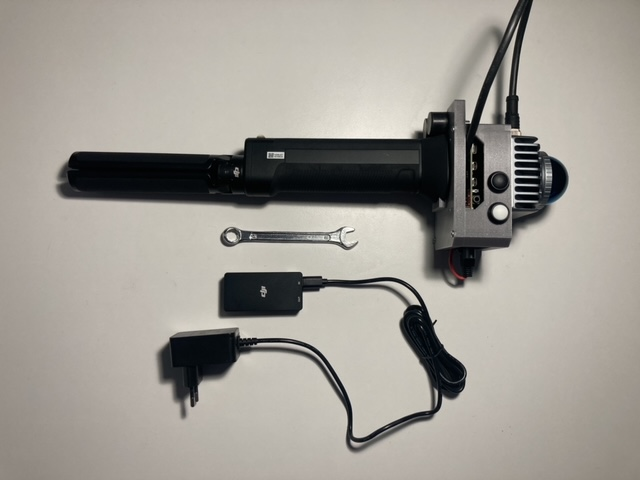
\includegraphics[width=\textwidth, angle = 90]{IMG_9478.jpg}
		\caption{MANDEYE DEV all components - 1: MANDEYE DEV, 2: Tool for nuts, 3: Charger.}
		\label{fig:m1}
	\end{subfigure}
	\hfill
	\begin{subfigure}[b]{0.7\textwidth}
		\centering
		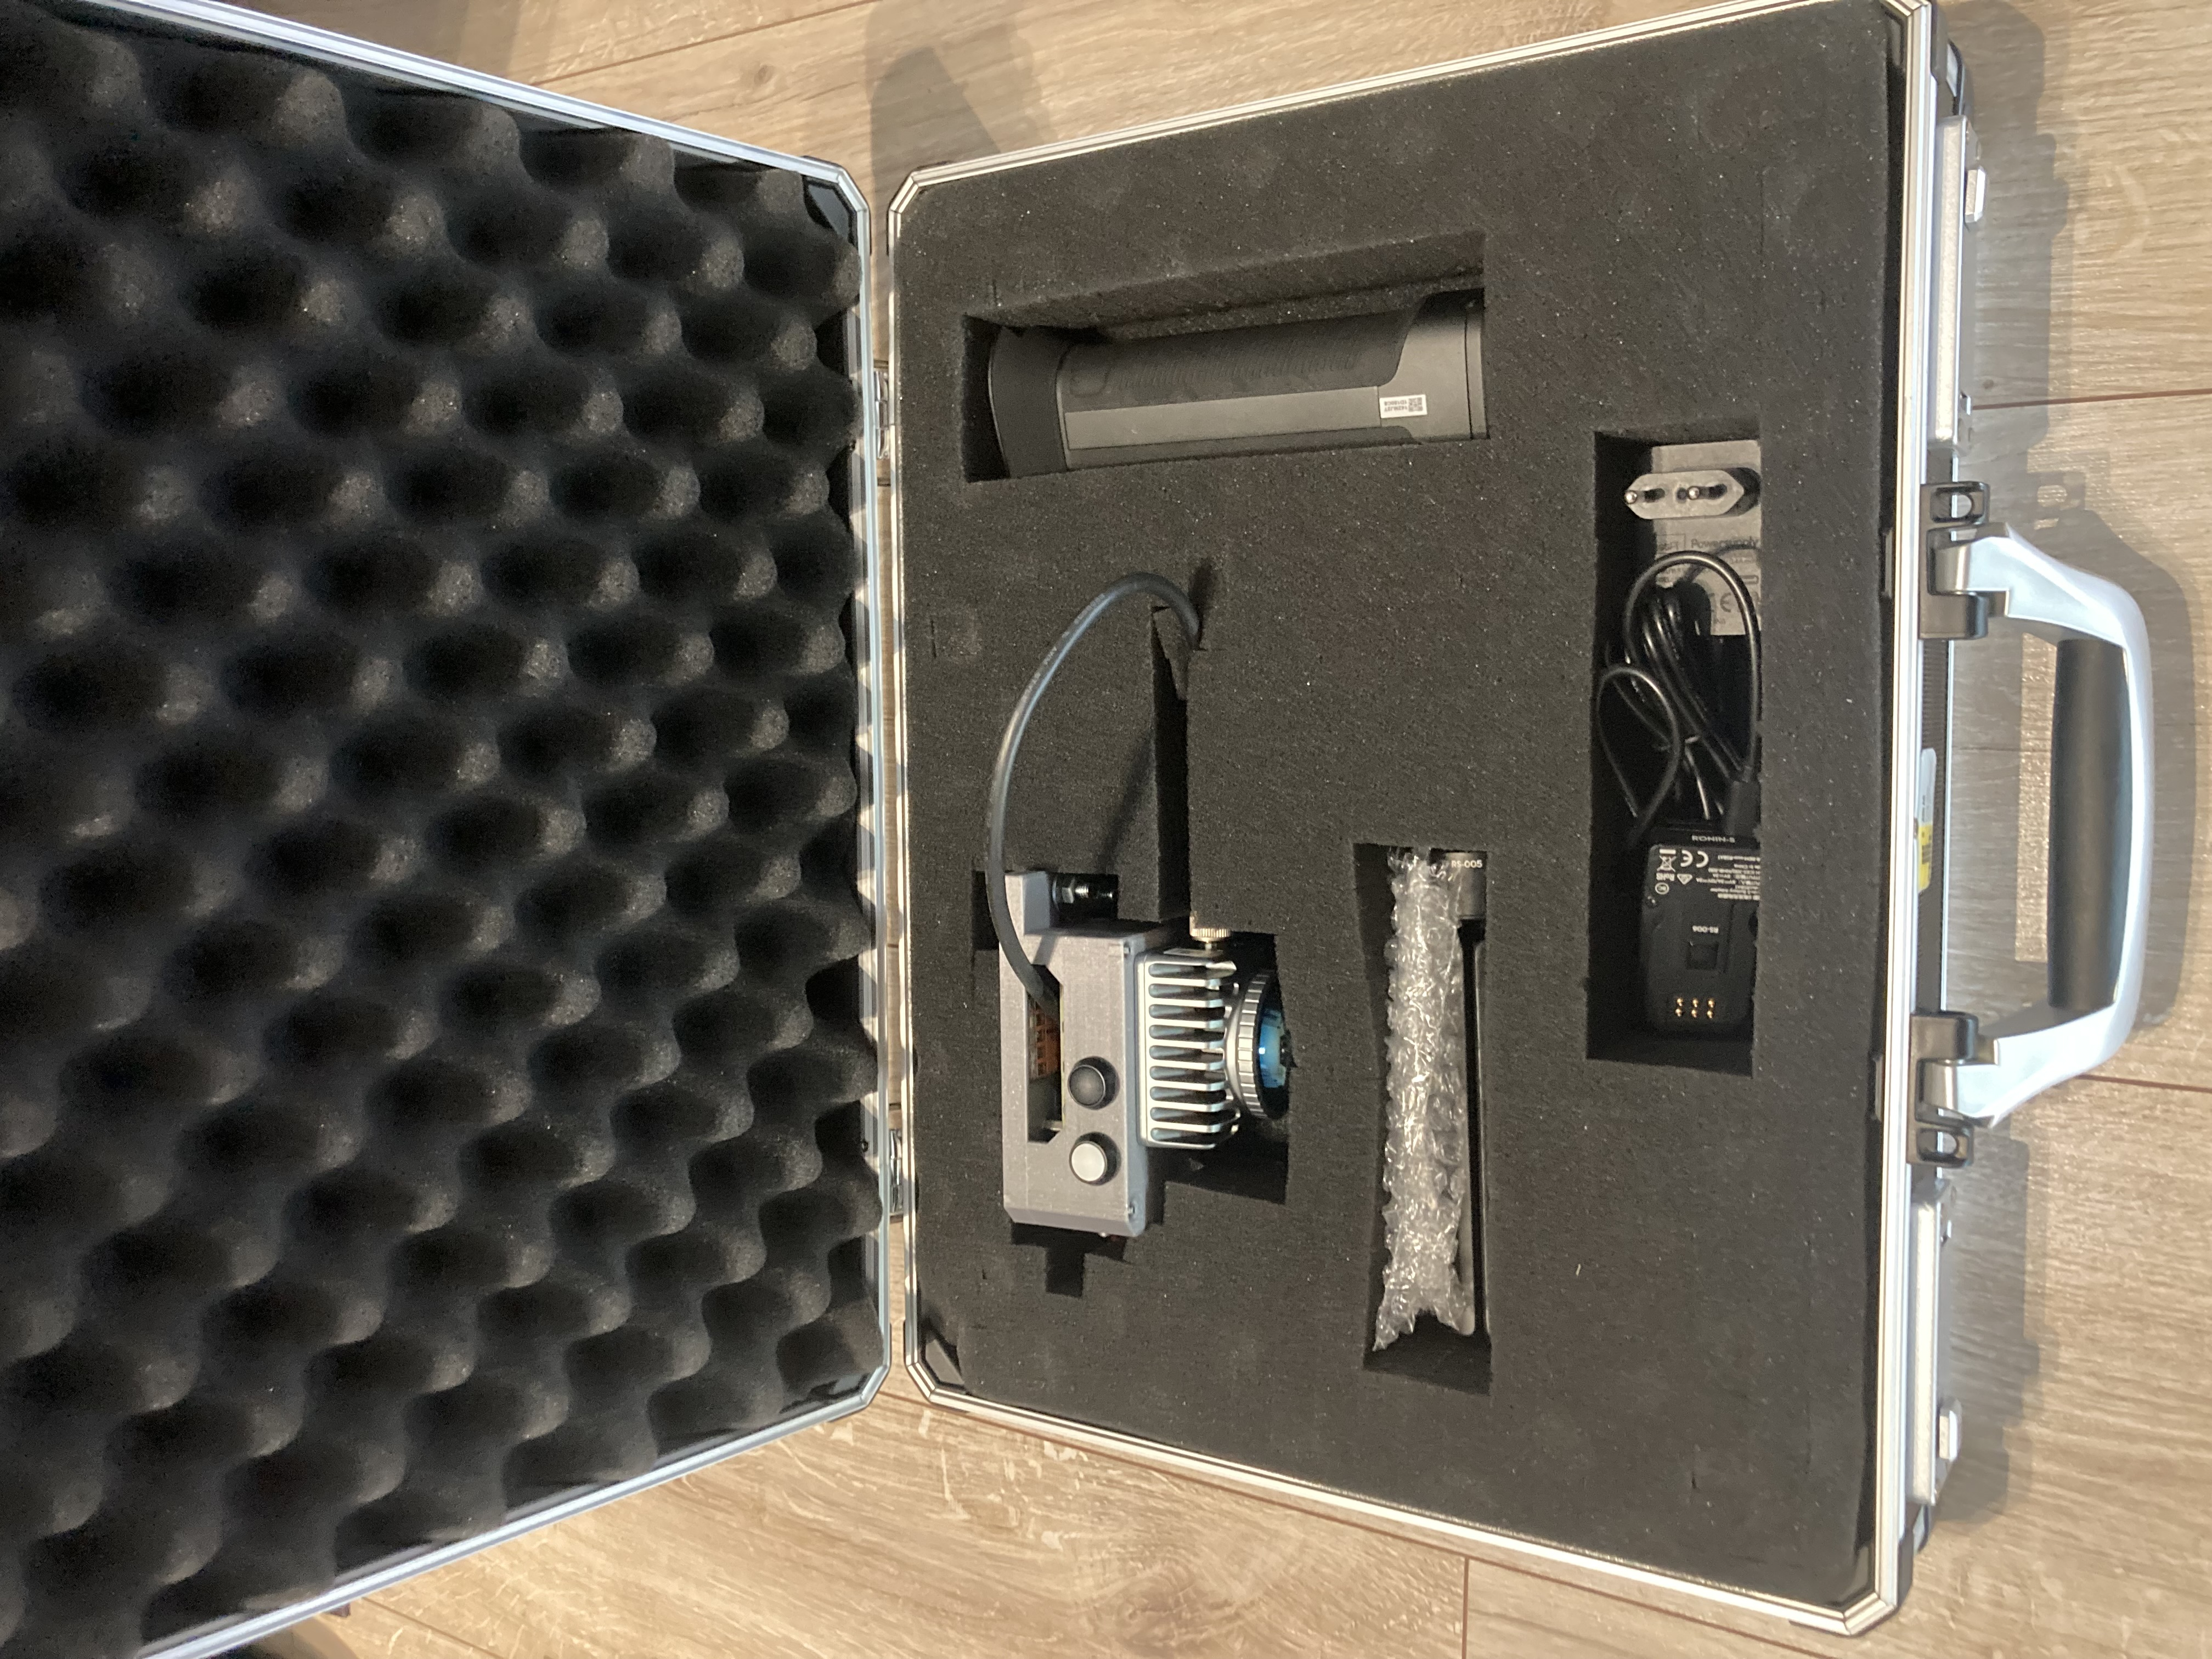
\includegraphics[width=\textwidth, angle = -90]{IMG_9493.jpg}
		\caption{Suitcase with MANDEYE DEV for secure transport.}
		\label{fig:m2}
	\end{subfigure}
	\caption{MANDEYE DEV ready for action.}
	\label{fig:mandeye_harware}
\end{figure}

\begin{figure}
	\centering
	\begin{subfigure}[b]{0.45\textwidth}
		\centering
		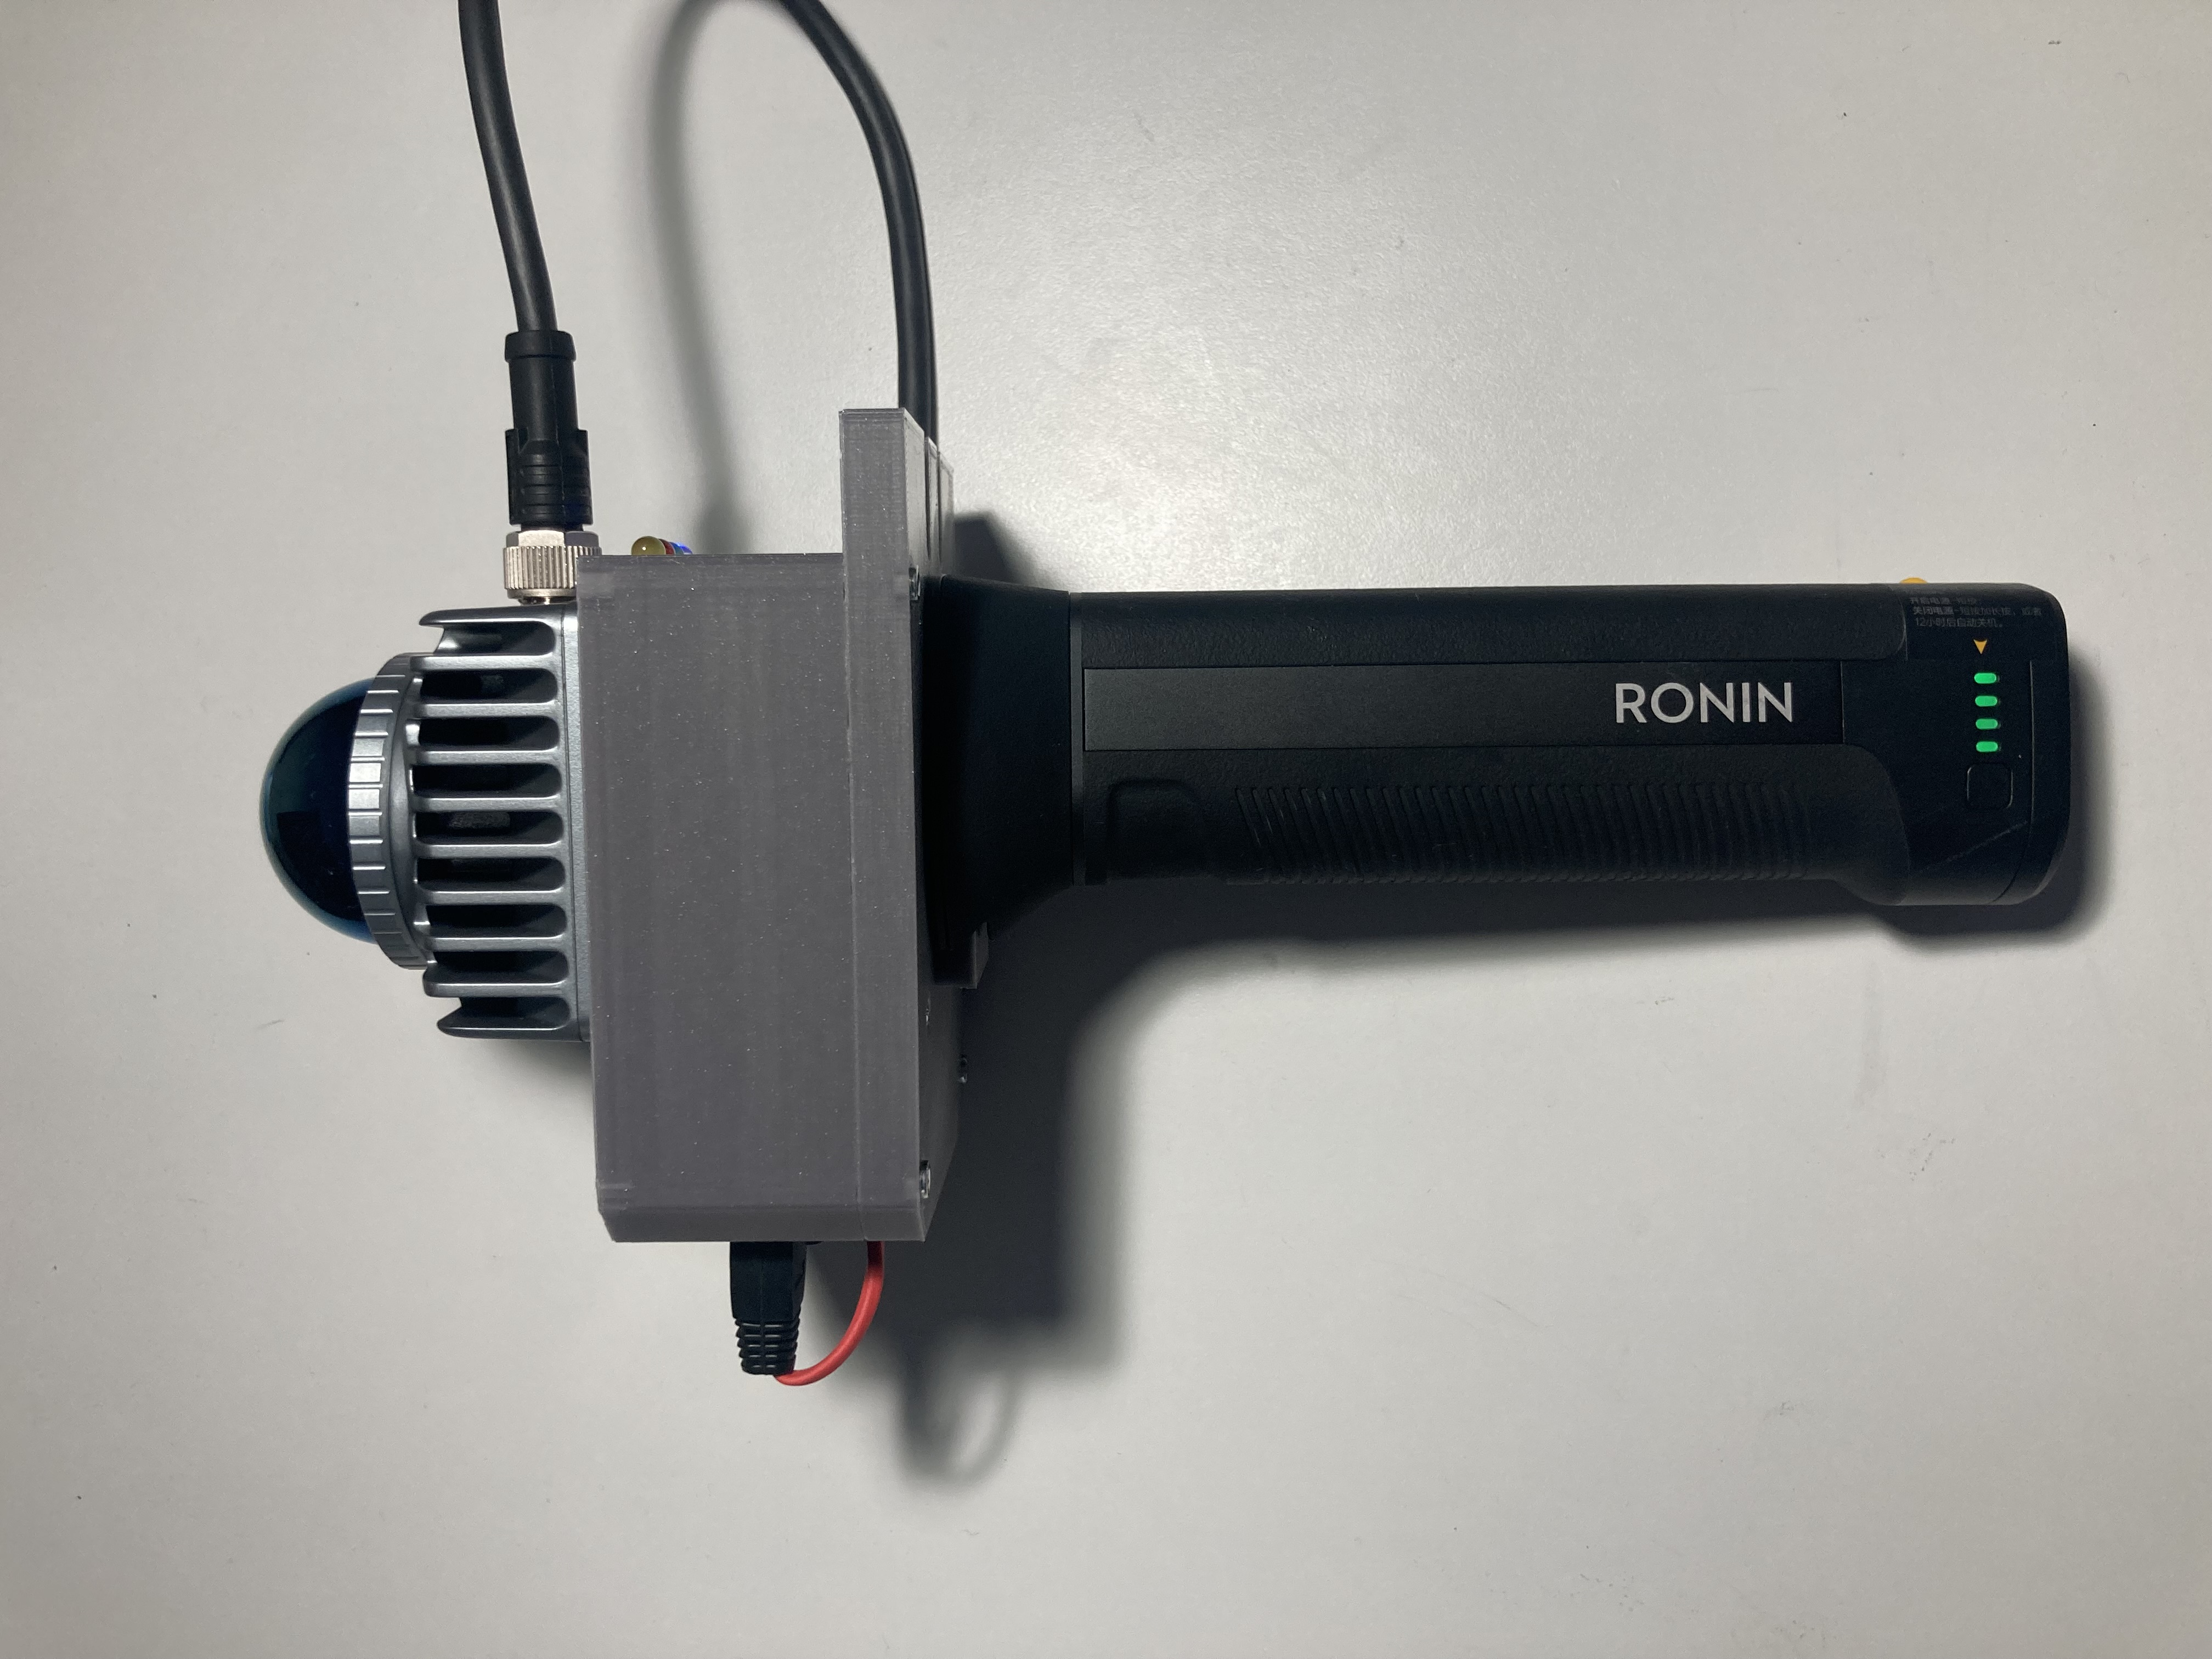
\includegraphics[width=\textwidth, angle = -90]{IMG_9482.jpg}
		\caption{STEP 1: Turn on: please click button on the bottom of the RONIN grip. Green square light should be visible.}
		\label{fig:m12}
	\end{subfigure}
	\hfill
	\begin{subfigure}[b]{0.45\textwidth}
		\centering
		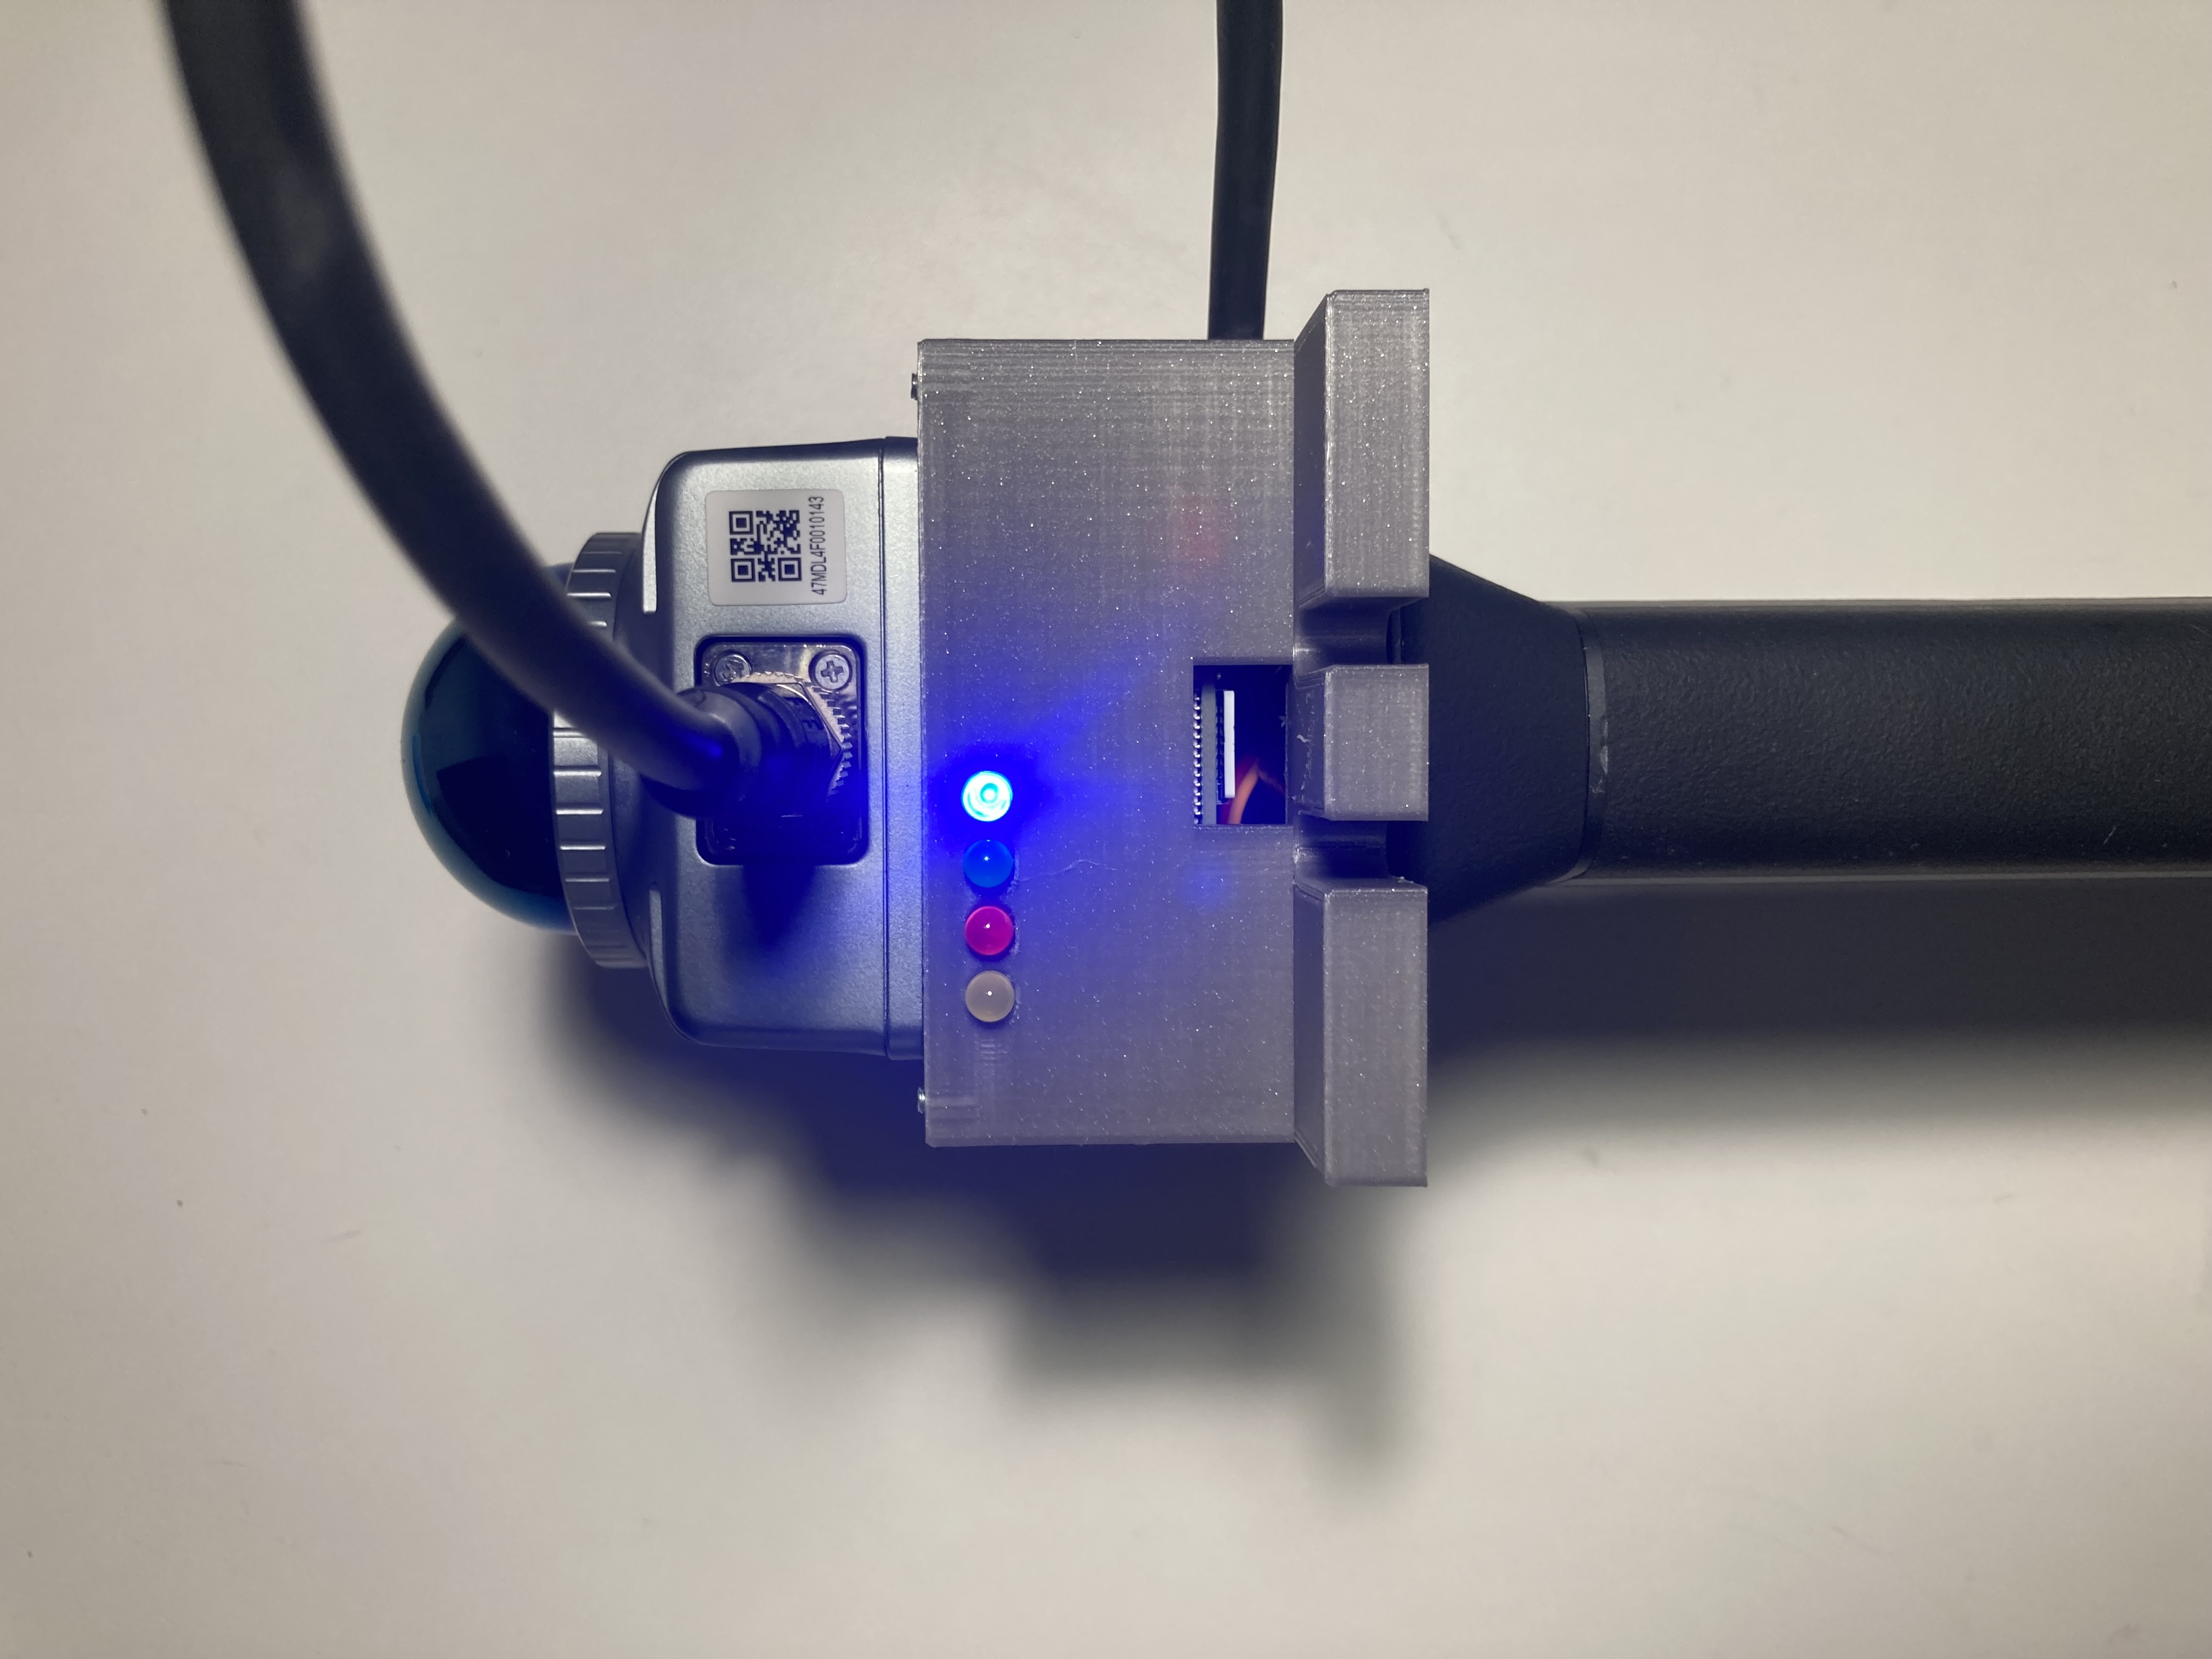
\includegraphics[width=\textwidth, angle = -90]{IMG_9484.jpg}
		\caption{STEP 2: Ones the MANDEYE DEV is turned on, it should turn on blue light.}
		\label{fig:m23}
	\end{subfigure}
	\hfill
	\begin{subfigure}[b]{0.45\textwidth}
		\centering
		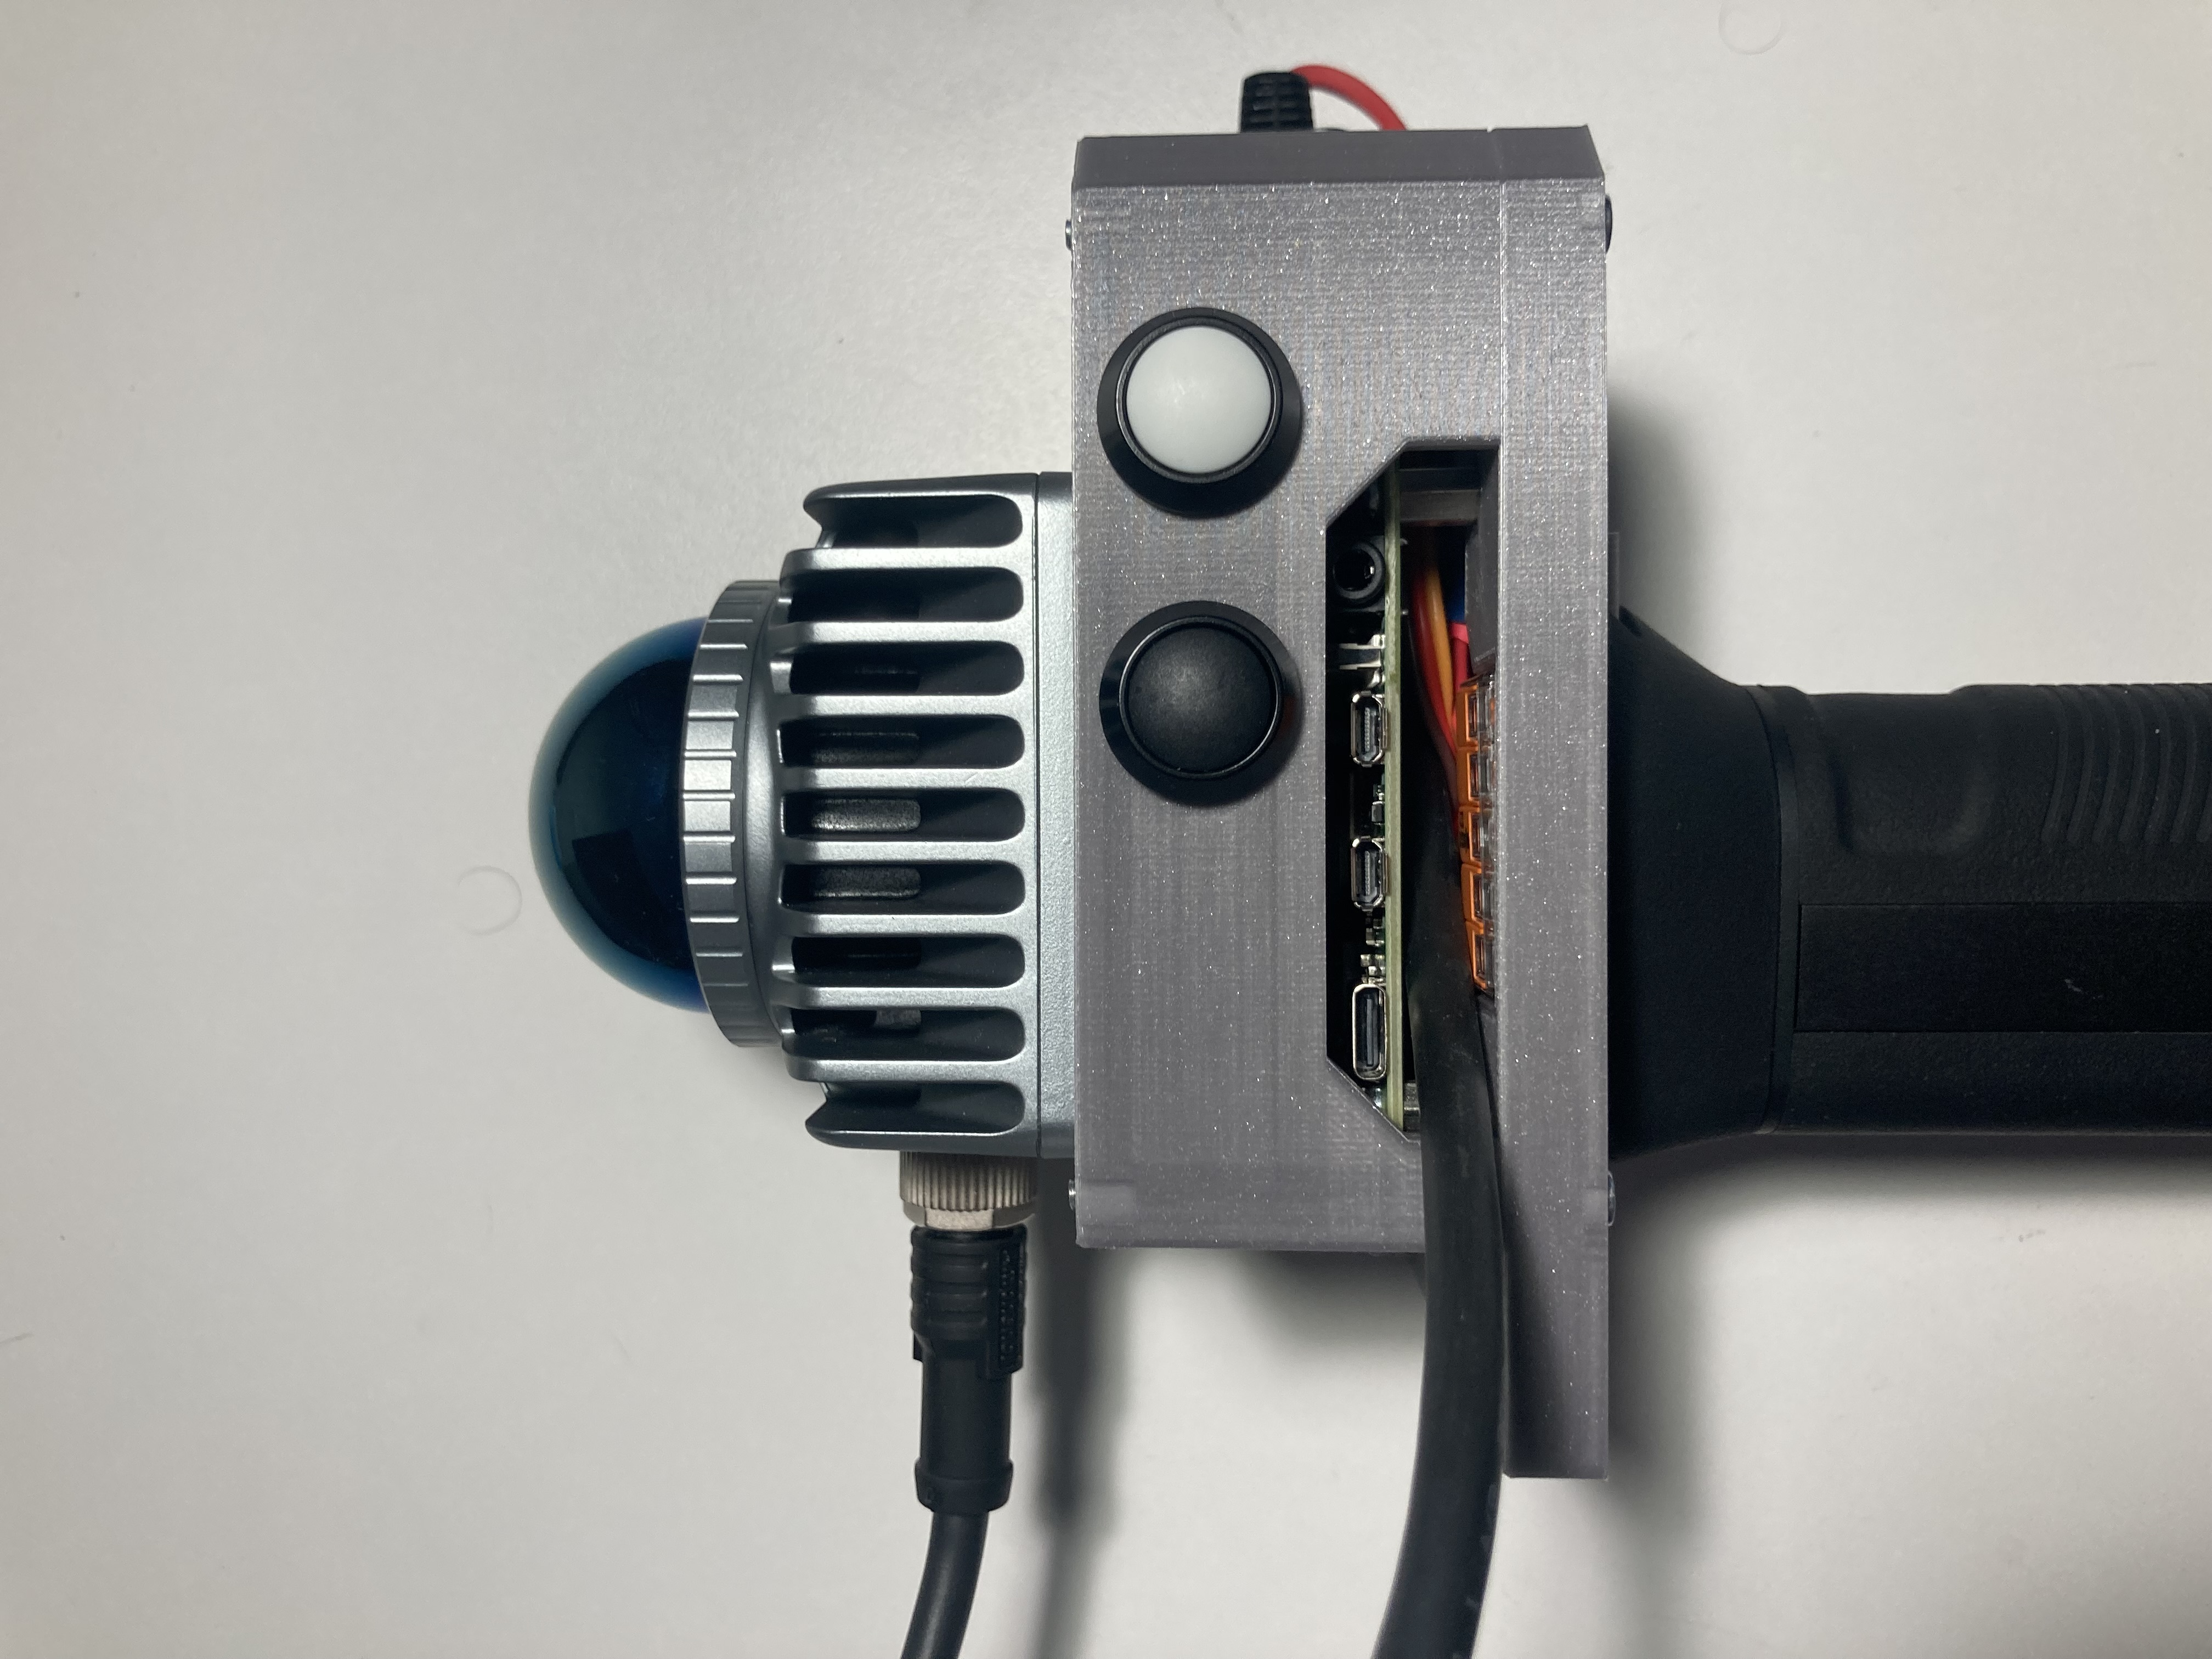
\includegraphics[width=\textwidth, angle = -90]{IMG_9481.jpg}
		\caption{STEP 3: Push white button for starting continuous scanning procedure.}
		\label{fig:m24}
	\end{subfigure}
	\hfill
	\begin{subfigure}[b]{0.45\textwidth}
		\centering
		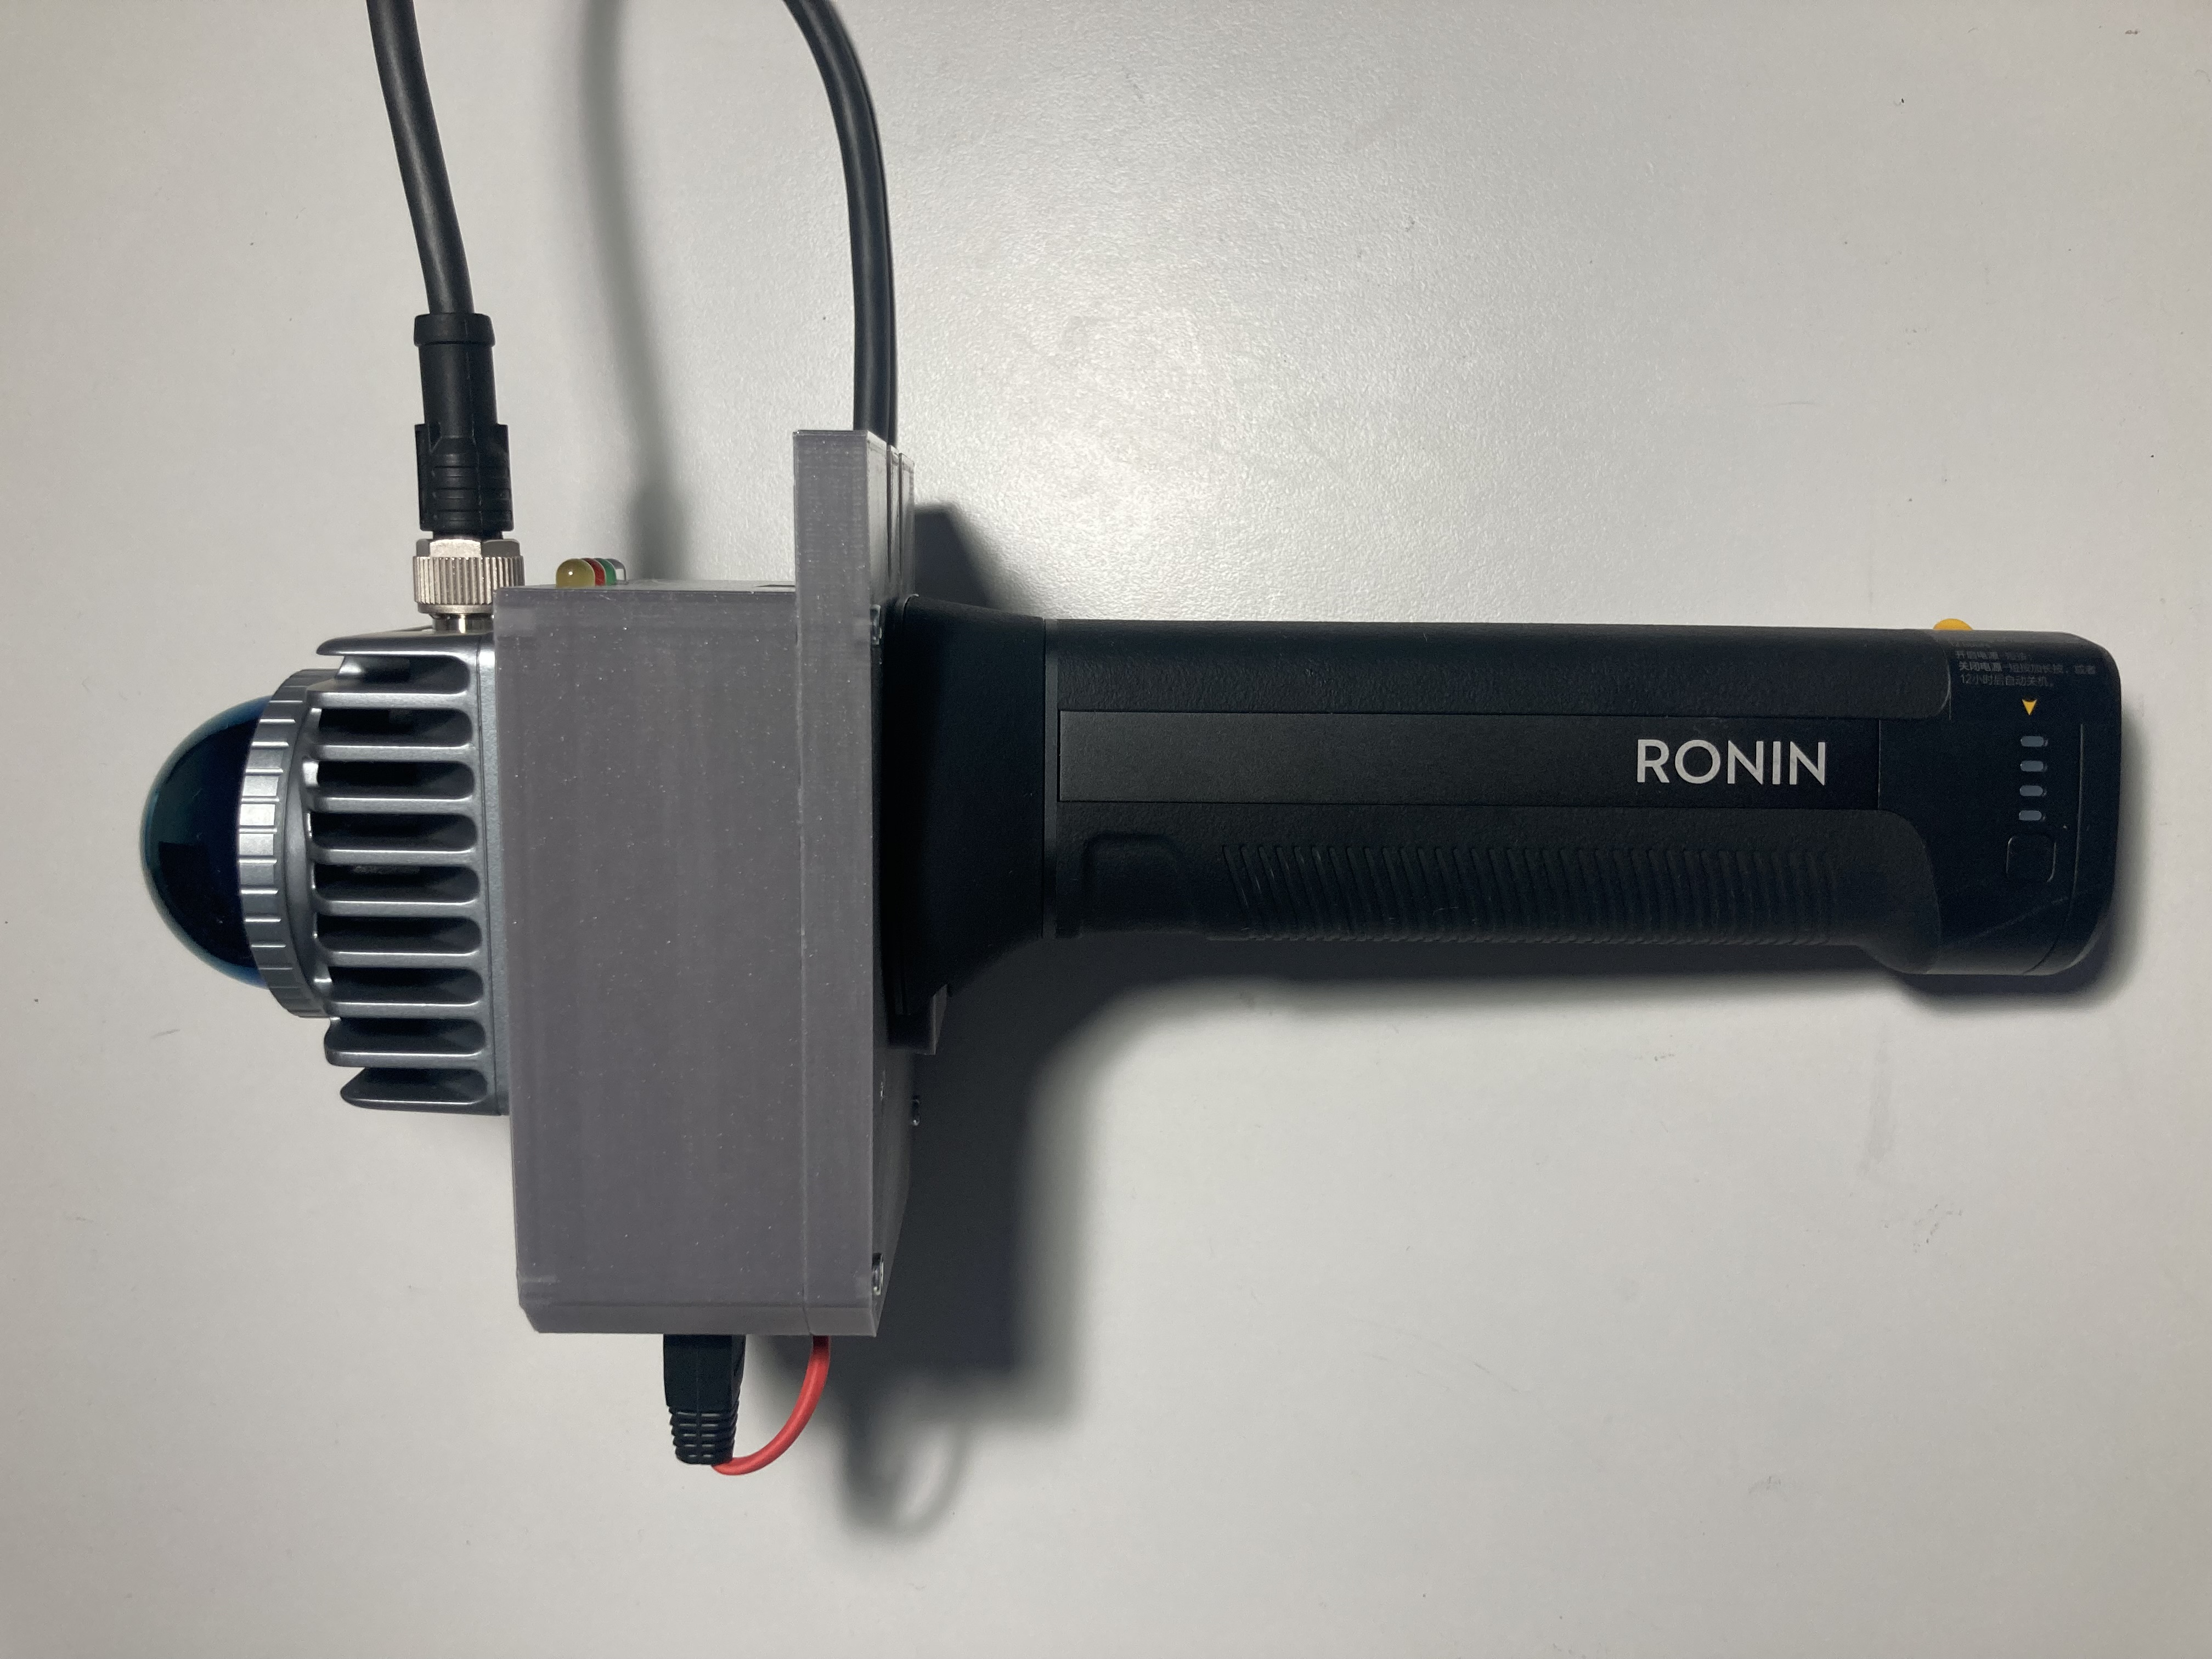
\includegraphics[width=\textwidth, angle = -90]{IMG_9483.jpg}
		\caption{STEP 4,5: To turn off continous scanning recordning press white button when red light is not lightning. Press shortly RONIN button and then press longer RONIN button. All RONIN lights should turn off.}
		\label{fig:m25}
	\end{subfigure}
	\caption{MANDEYE DEV ready for action.}
	\label{fig:mandeye_harware2}
\end{figure}

\begin{figure}
	\centering
	\begin{subfigure}[b]{0.45\textwidth}
		\centering
		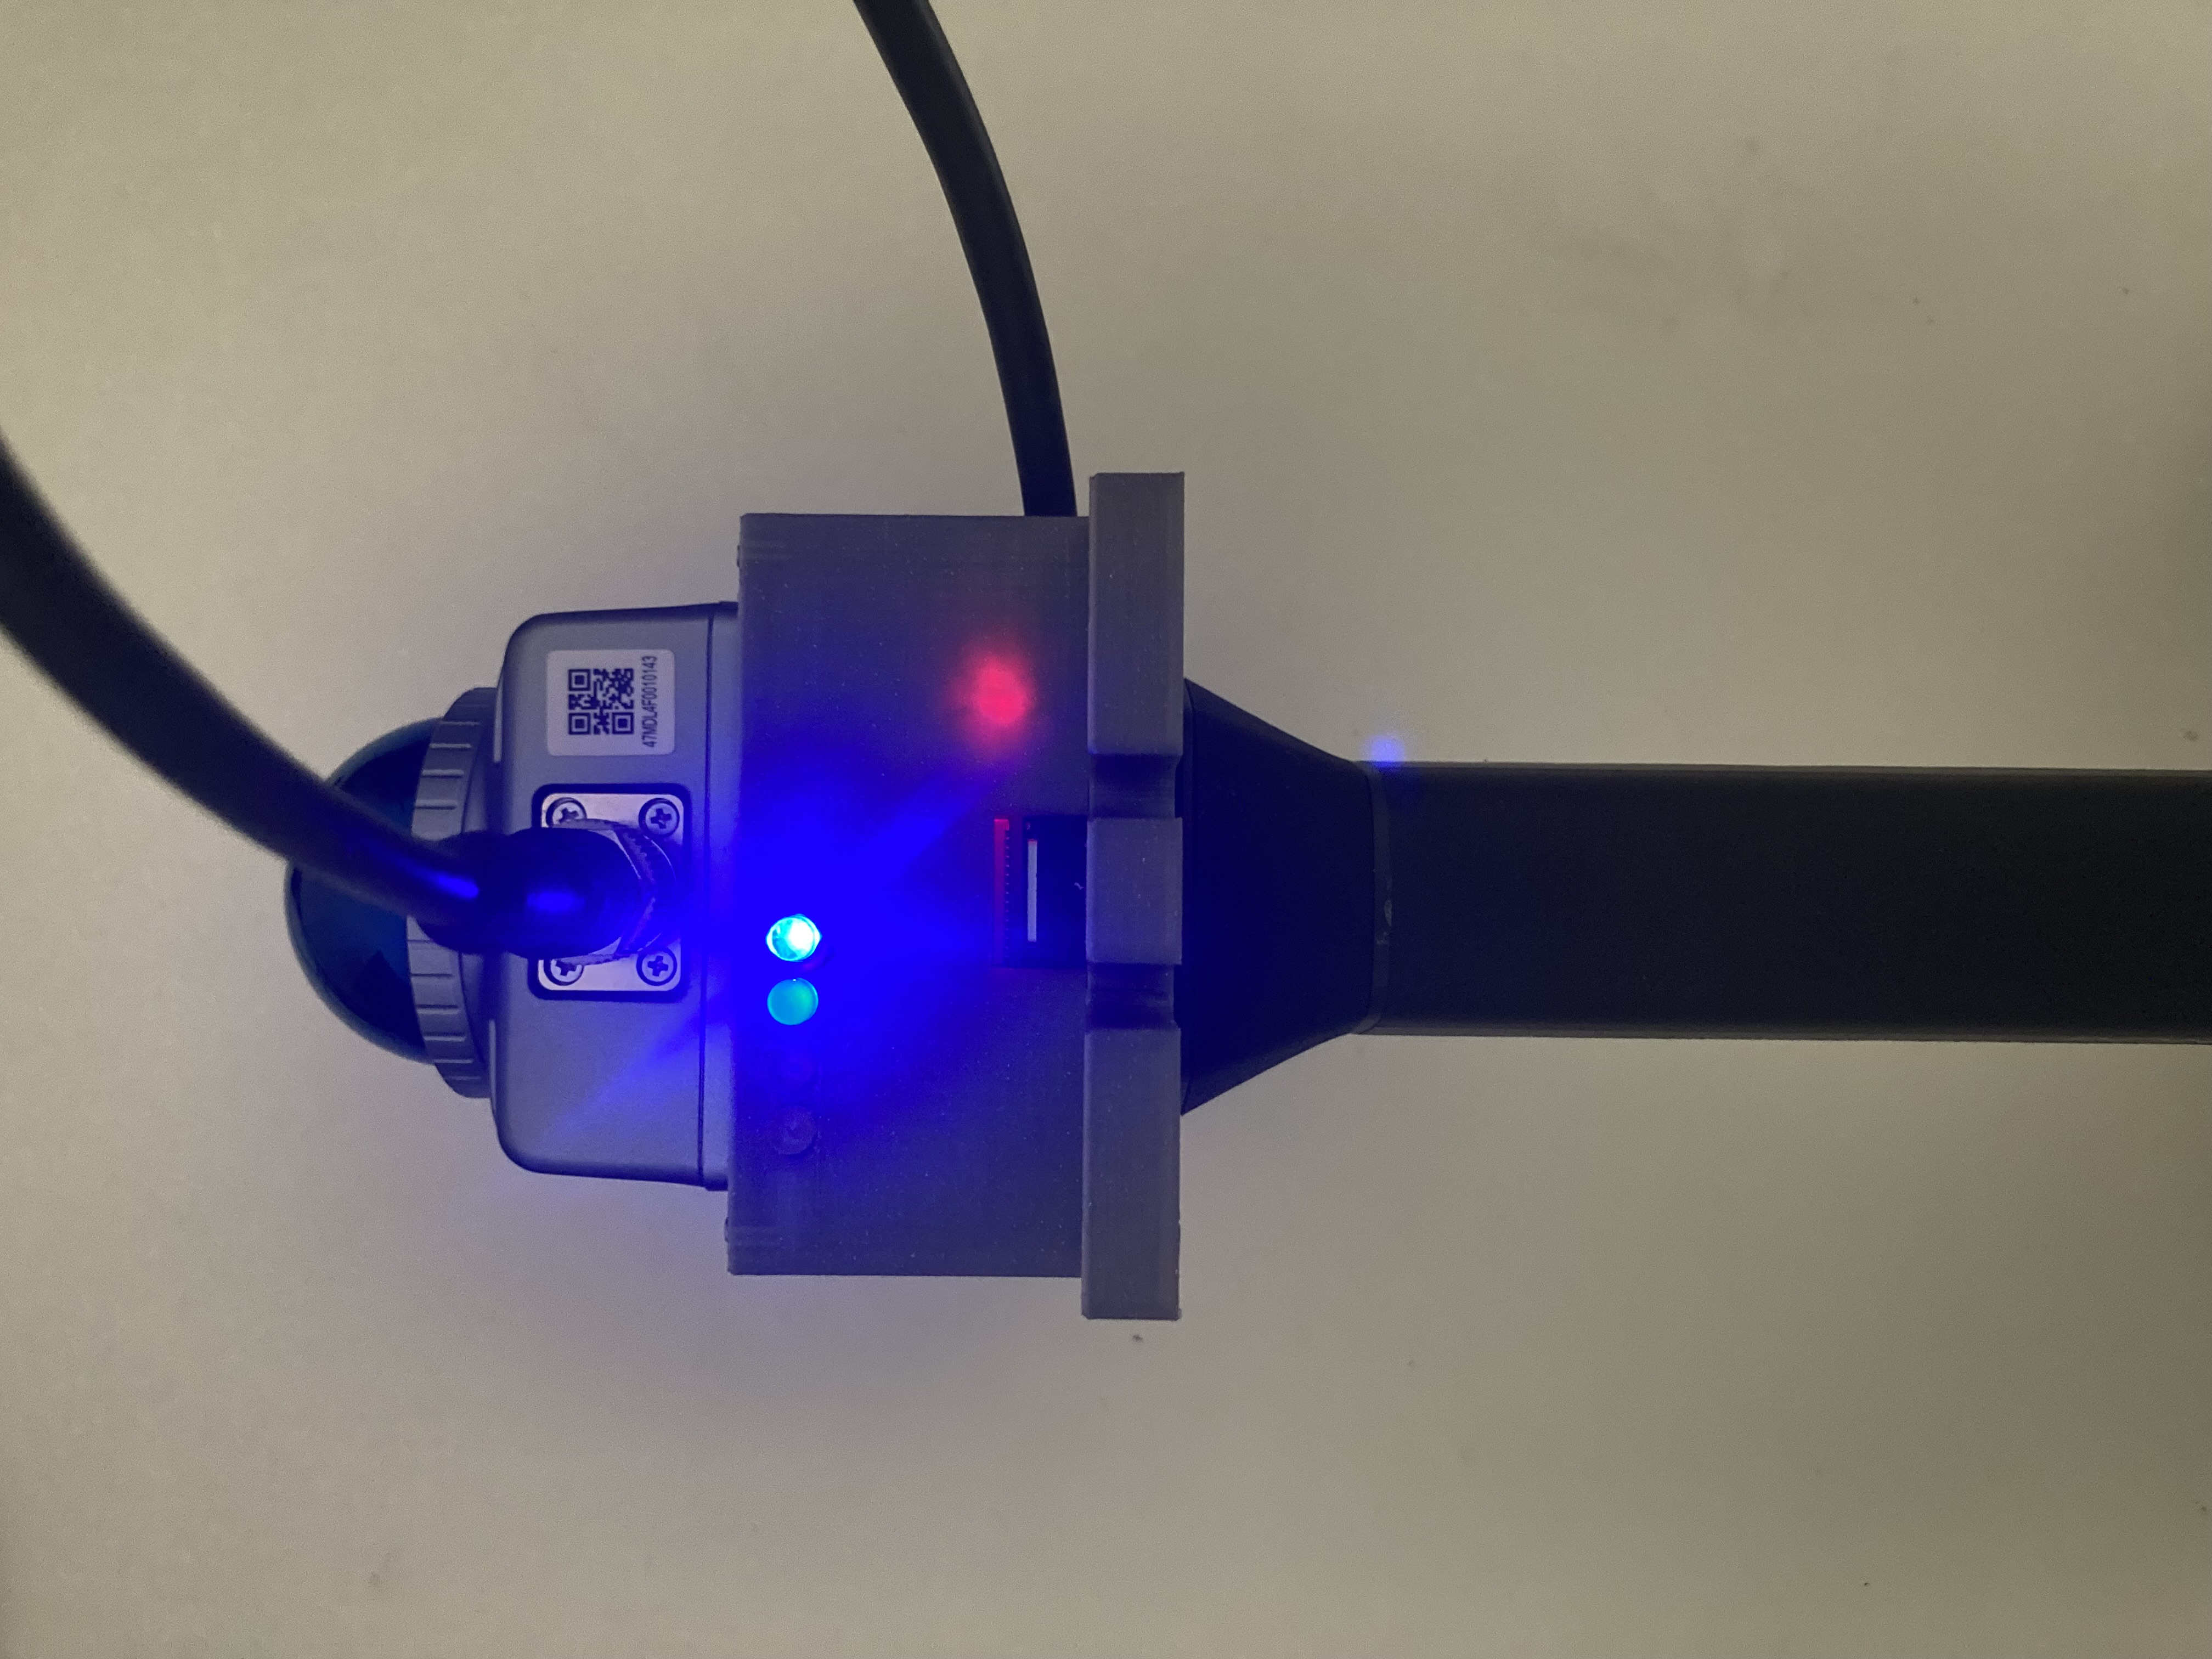
\includegraphics[width=\textwidth, angle = -90]{IMG_9494.jpg}
		\caption{MANDEYE DEV is showing by green light that 3D continuous scanning data are recorded in local memory.}
		\label{fig:m16}
	\end{subfigure}
	\hfill
	\begin{subfigure}[b]{0.45\textwidth}
		\centering
		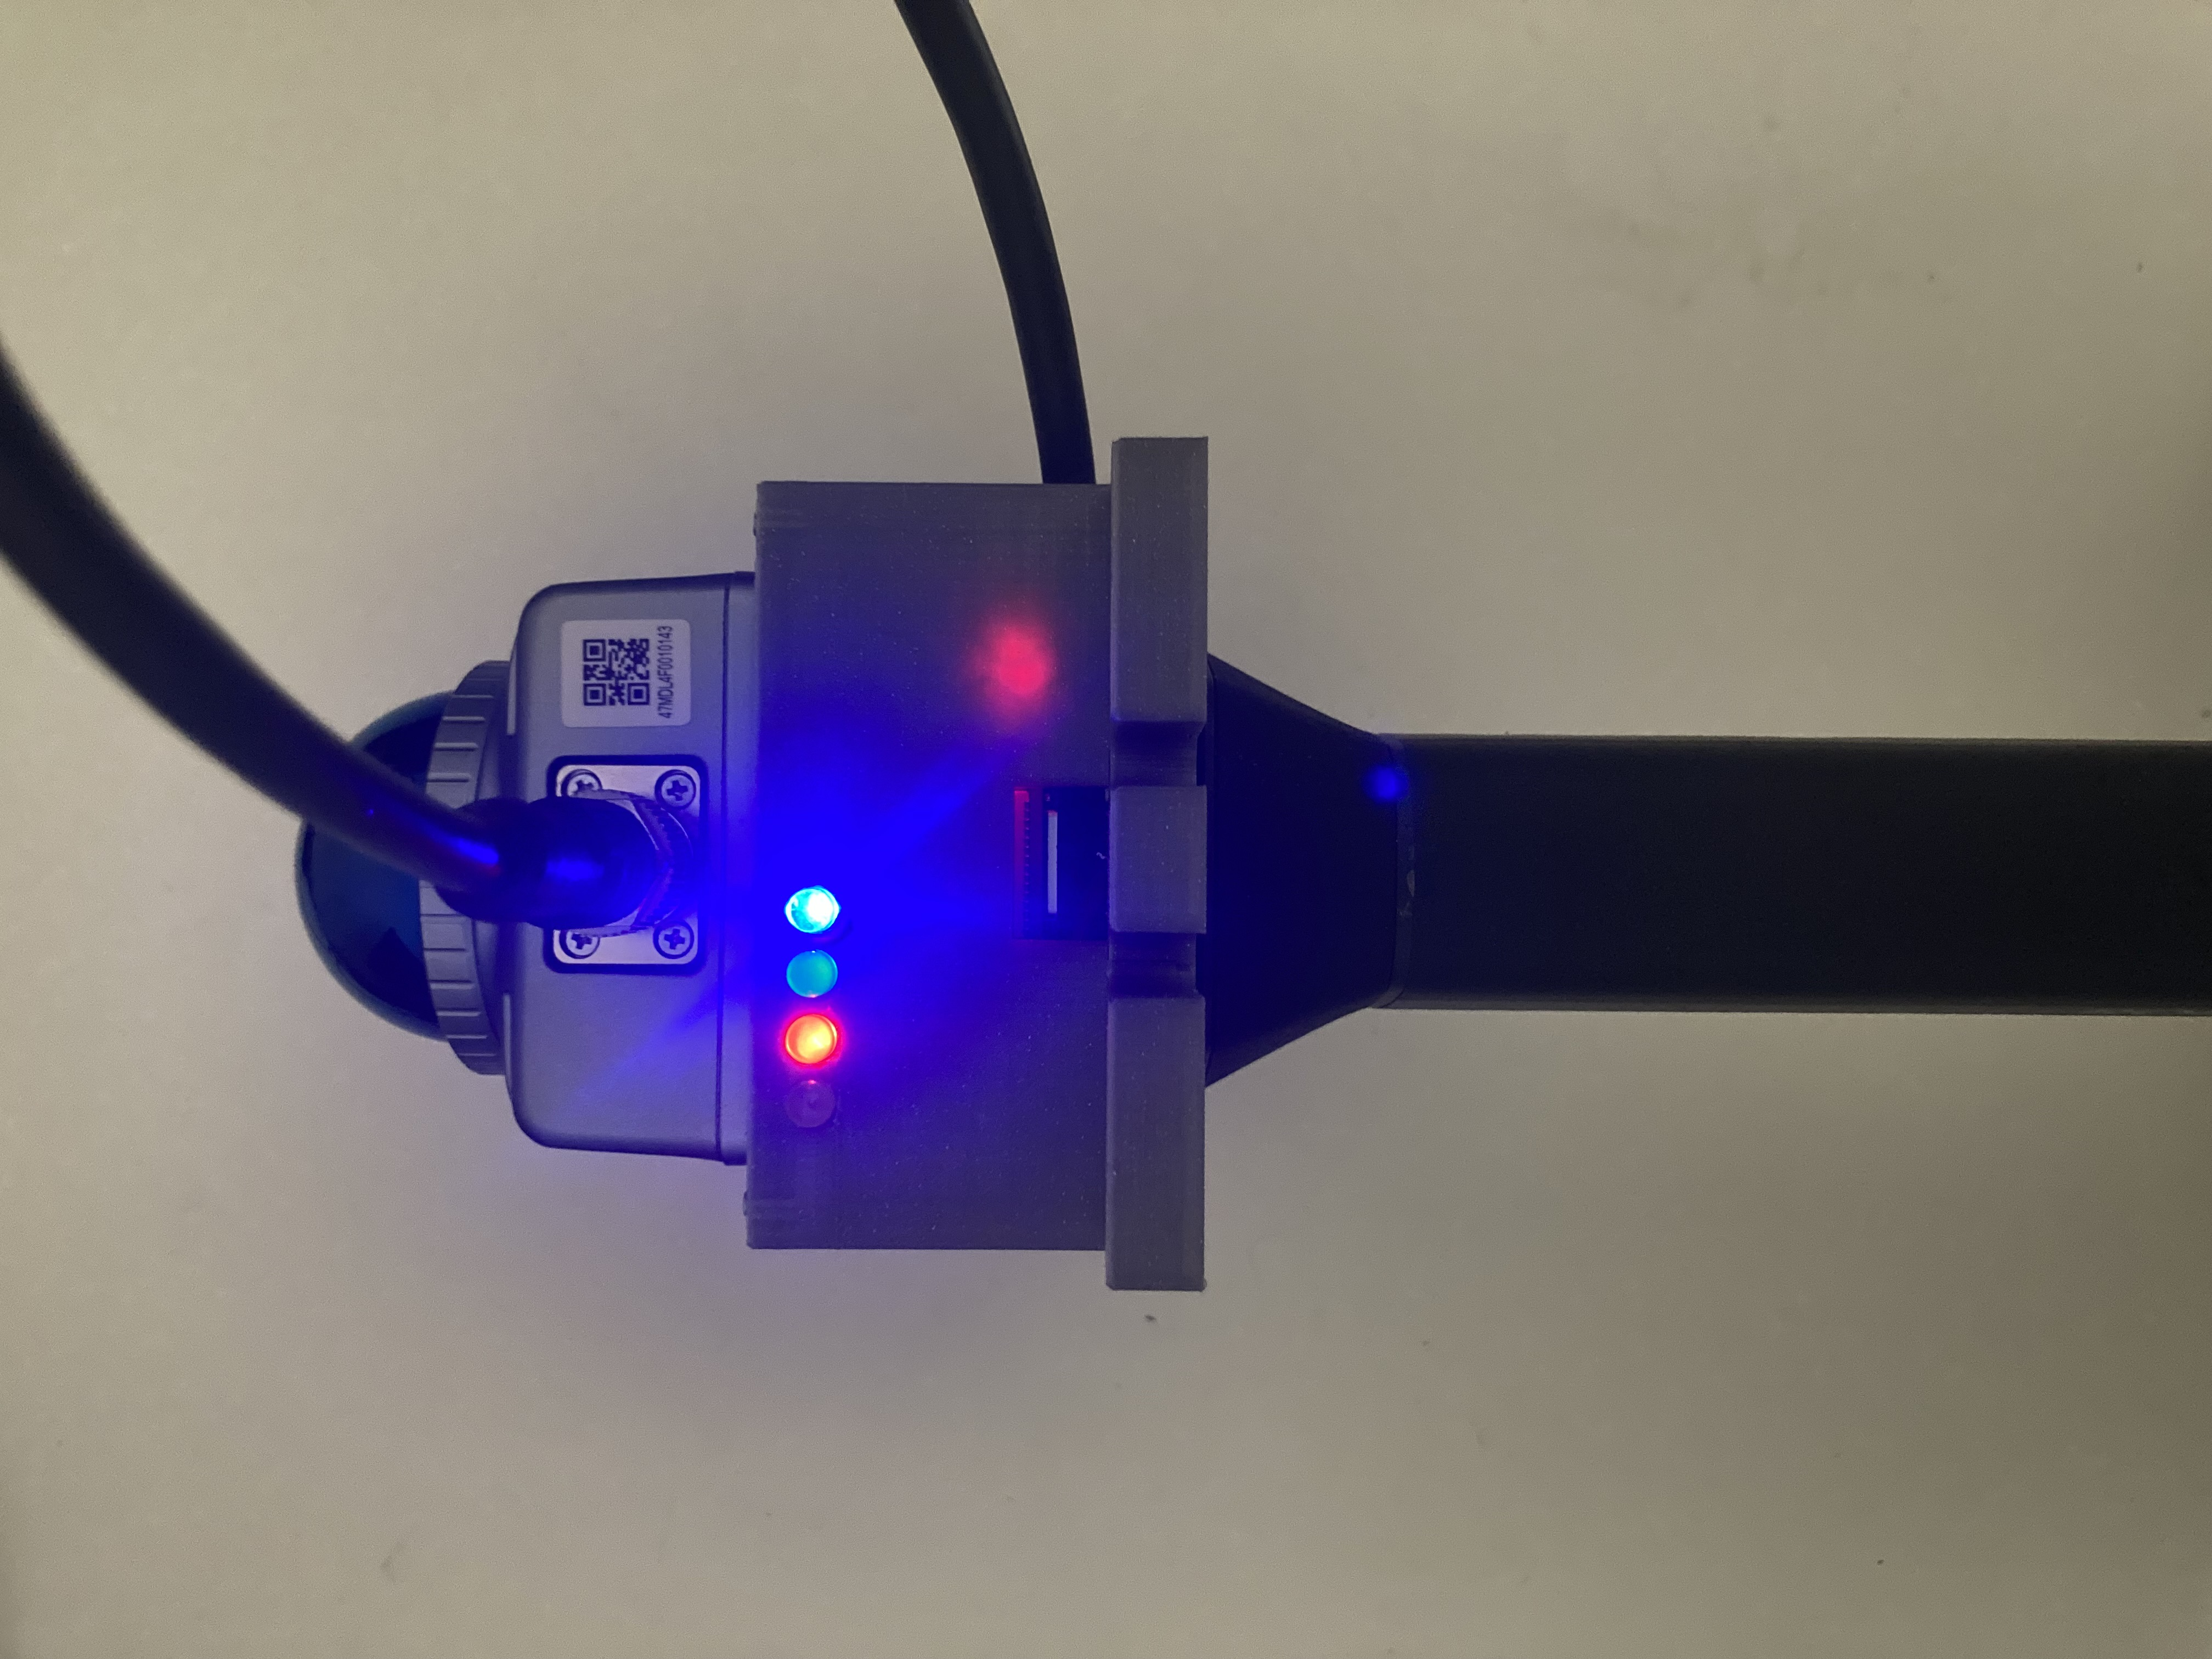
\includegraphics[width=\textwidth, angle = -90]{IMG_9495.jpg}
		\caption{MANDEYE DEV is showing by green and red light that it copies continuous scanning data from local memory to USB stick.}
		\label{fig:m26}
	\end{subfigure}
	\caption{MANDEYE DEV during continuous scanning.}
	\label{fig:mandeye_harware3}
\end{figure}

\begin{figure}
	\centering
	\begin{subfigure}[b]{0.45\textwidth}
		\centering
		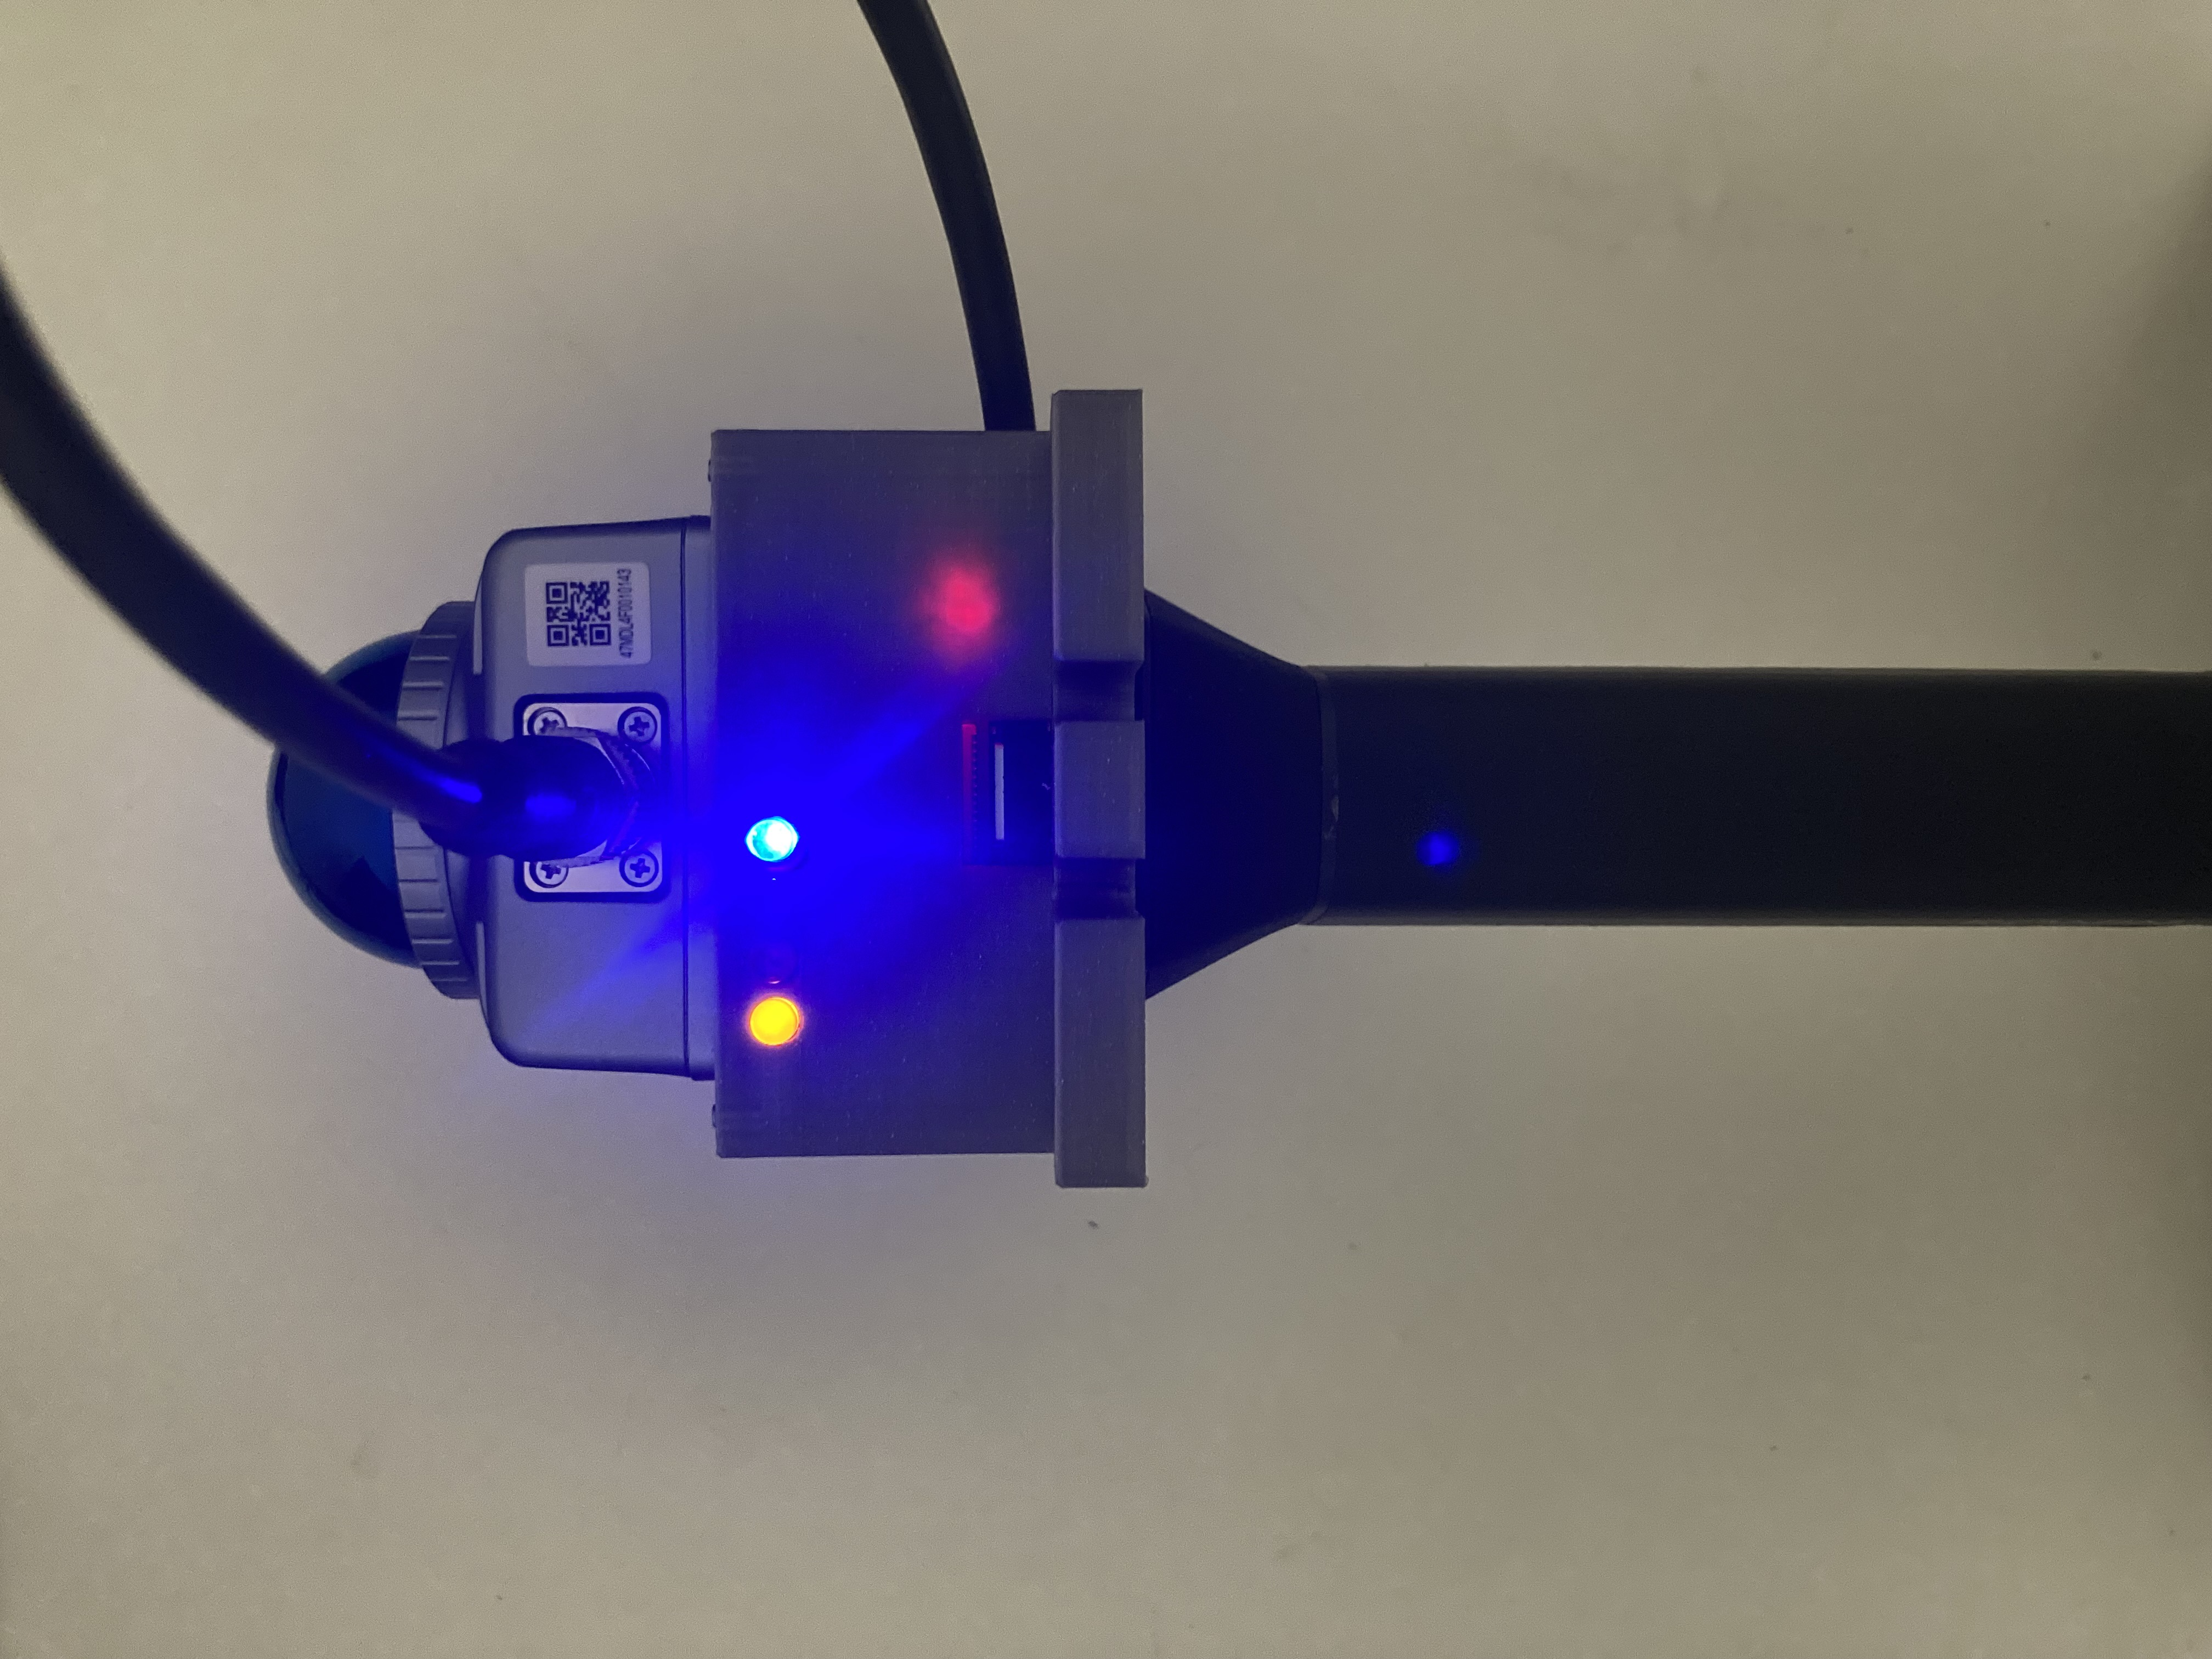
\includegraphics[width=\textwidth, angle = -90]{IMG_9498.jpg}
		\caption{MANDEYE DEV is showing by yellow light that 3D data are recorded in local memory.}
		\label{fig:m17}
	\end{subfigure}
	\hfill
	\begin{subfigure}[b]{0.45\textwidth}
		\centering
		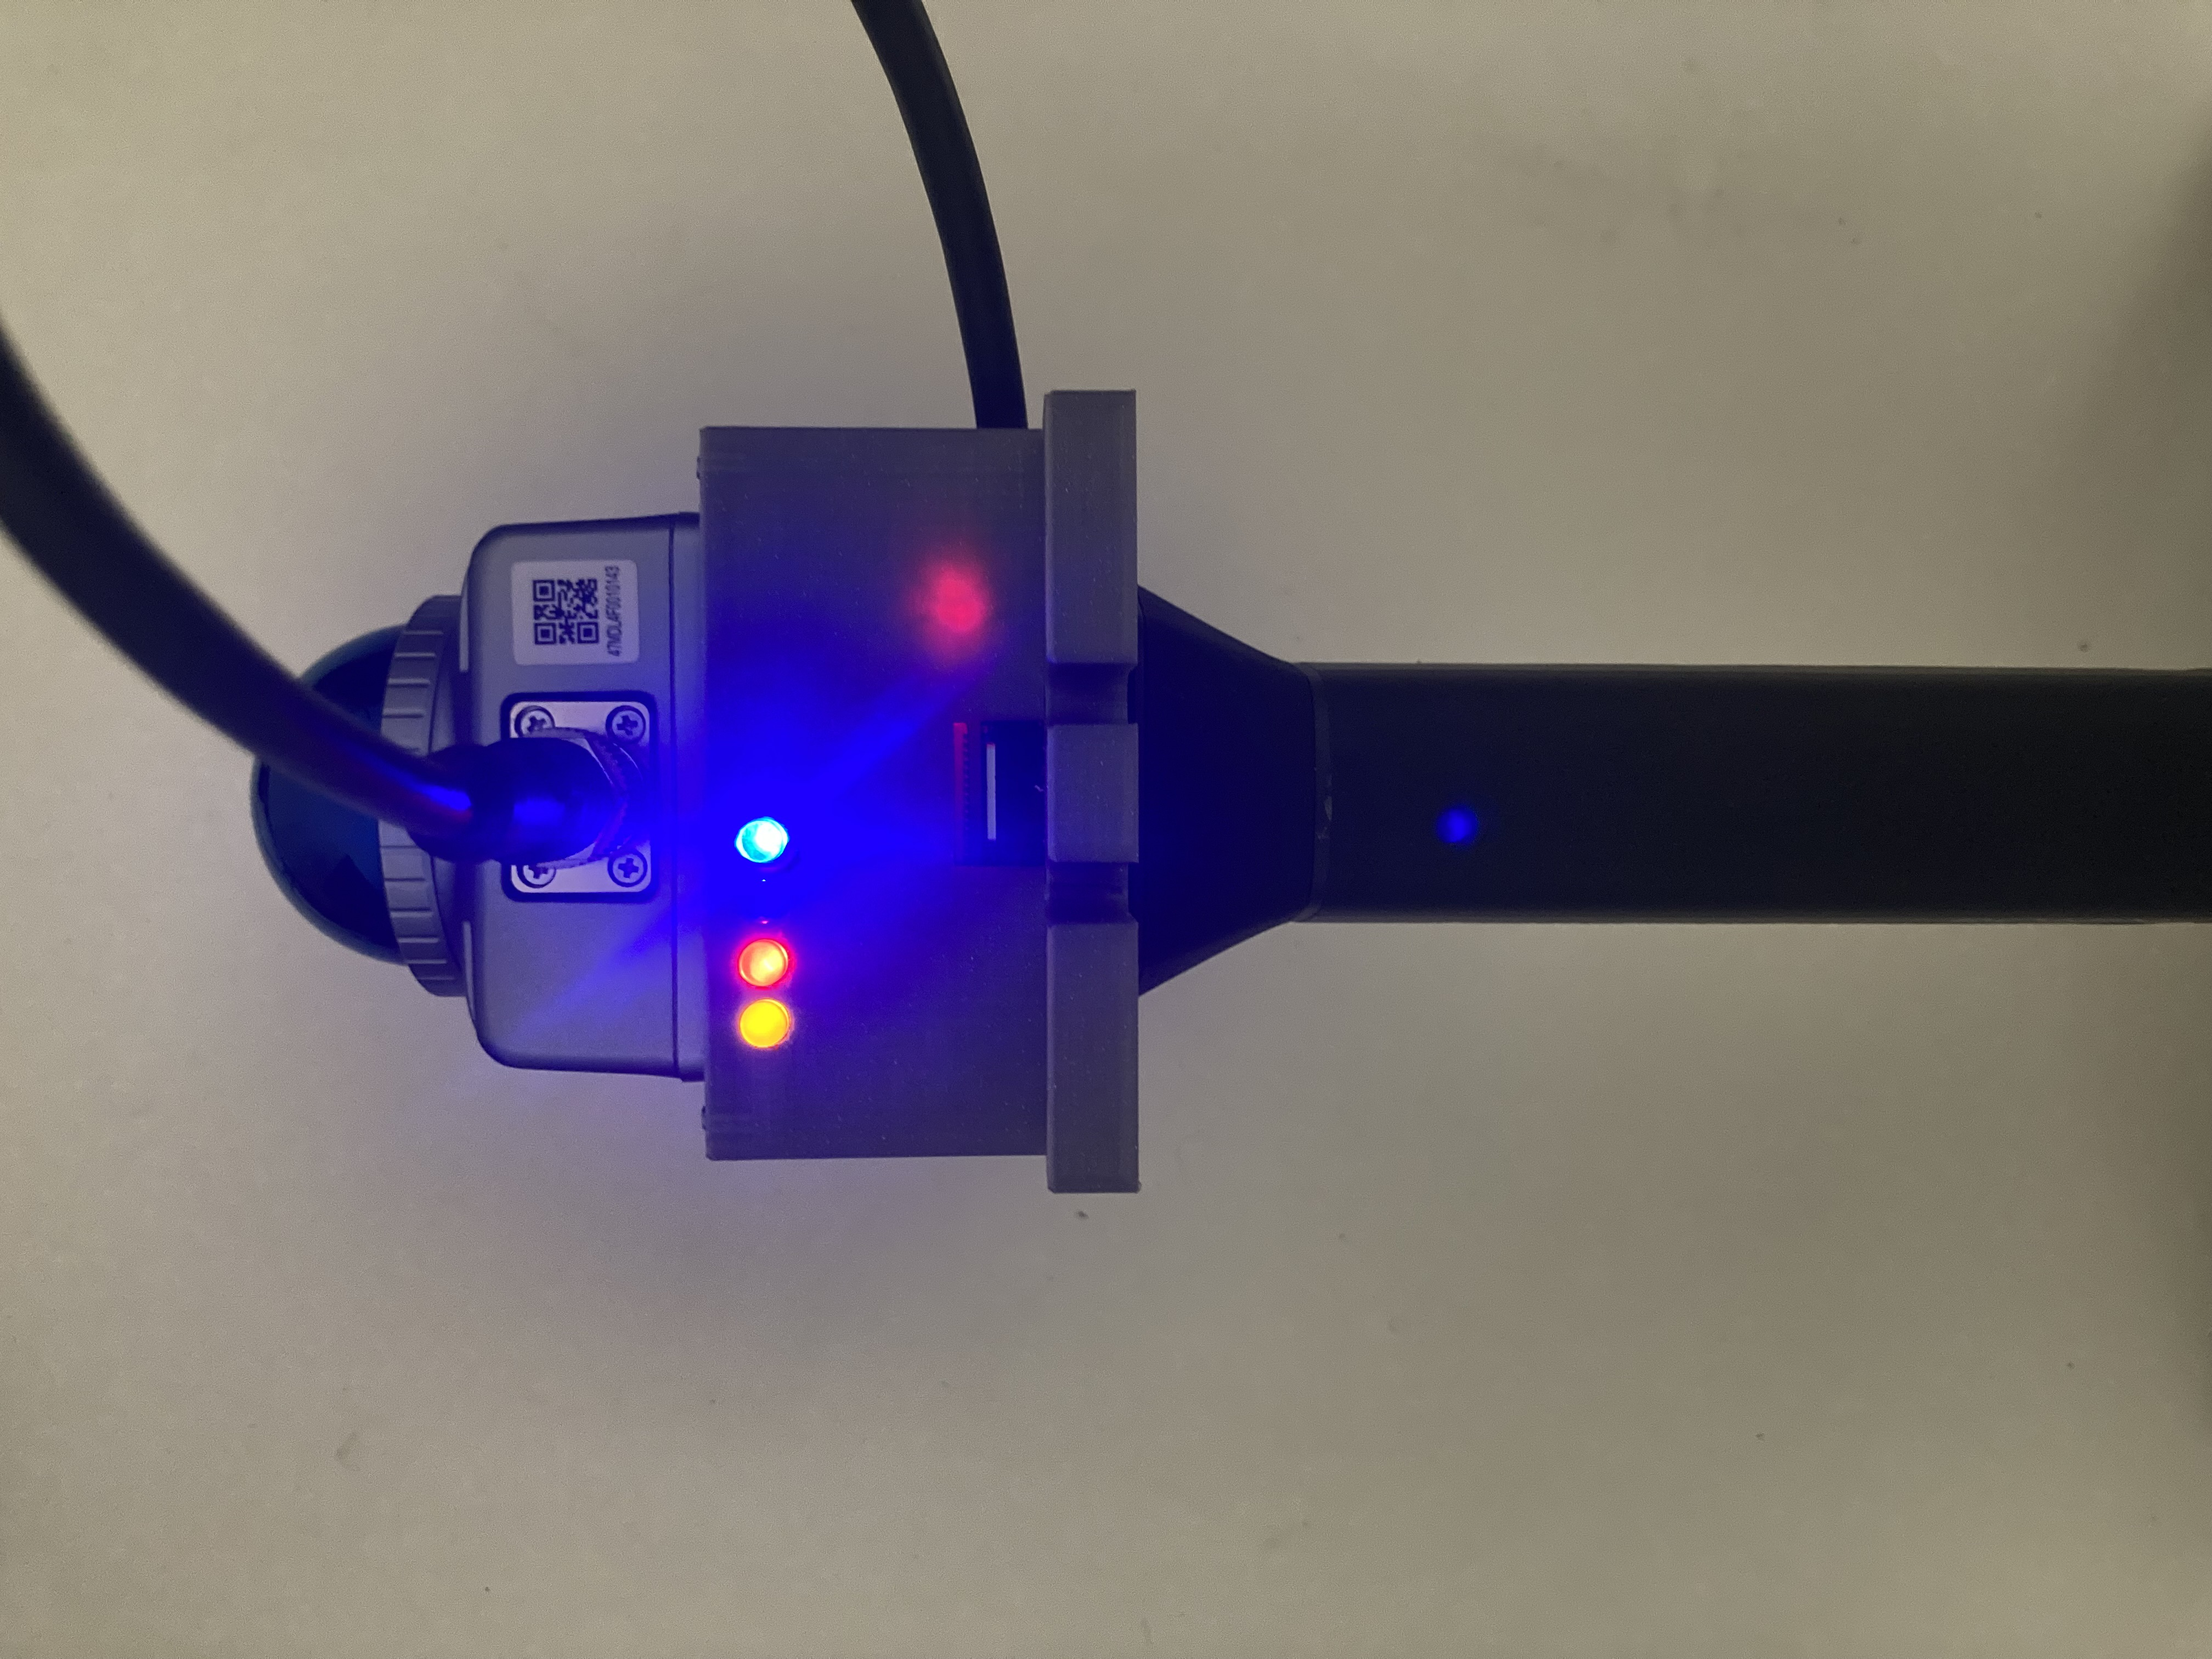
\includegraphics[width=\textwidth, angle = -90]{IMG_9499.jpg}
		\caption{MANDEYE DEV is showing by yellow and red light that it copies data from local memory to USB stick.}
		\label{fig:m27}
	\end{subfigure}
	\caption{MANDEYE DEV during stop/scan scanning.}
	\label{fig:mandeye_harware4}
\end{figure}

\begin{figure}
	\centering
	\begin{subfigure}[b]{0.45\textwidth}
		\centering
		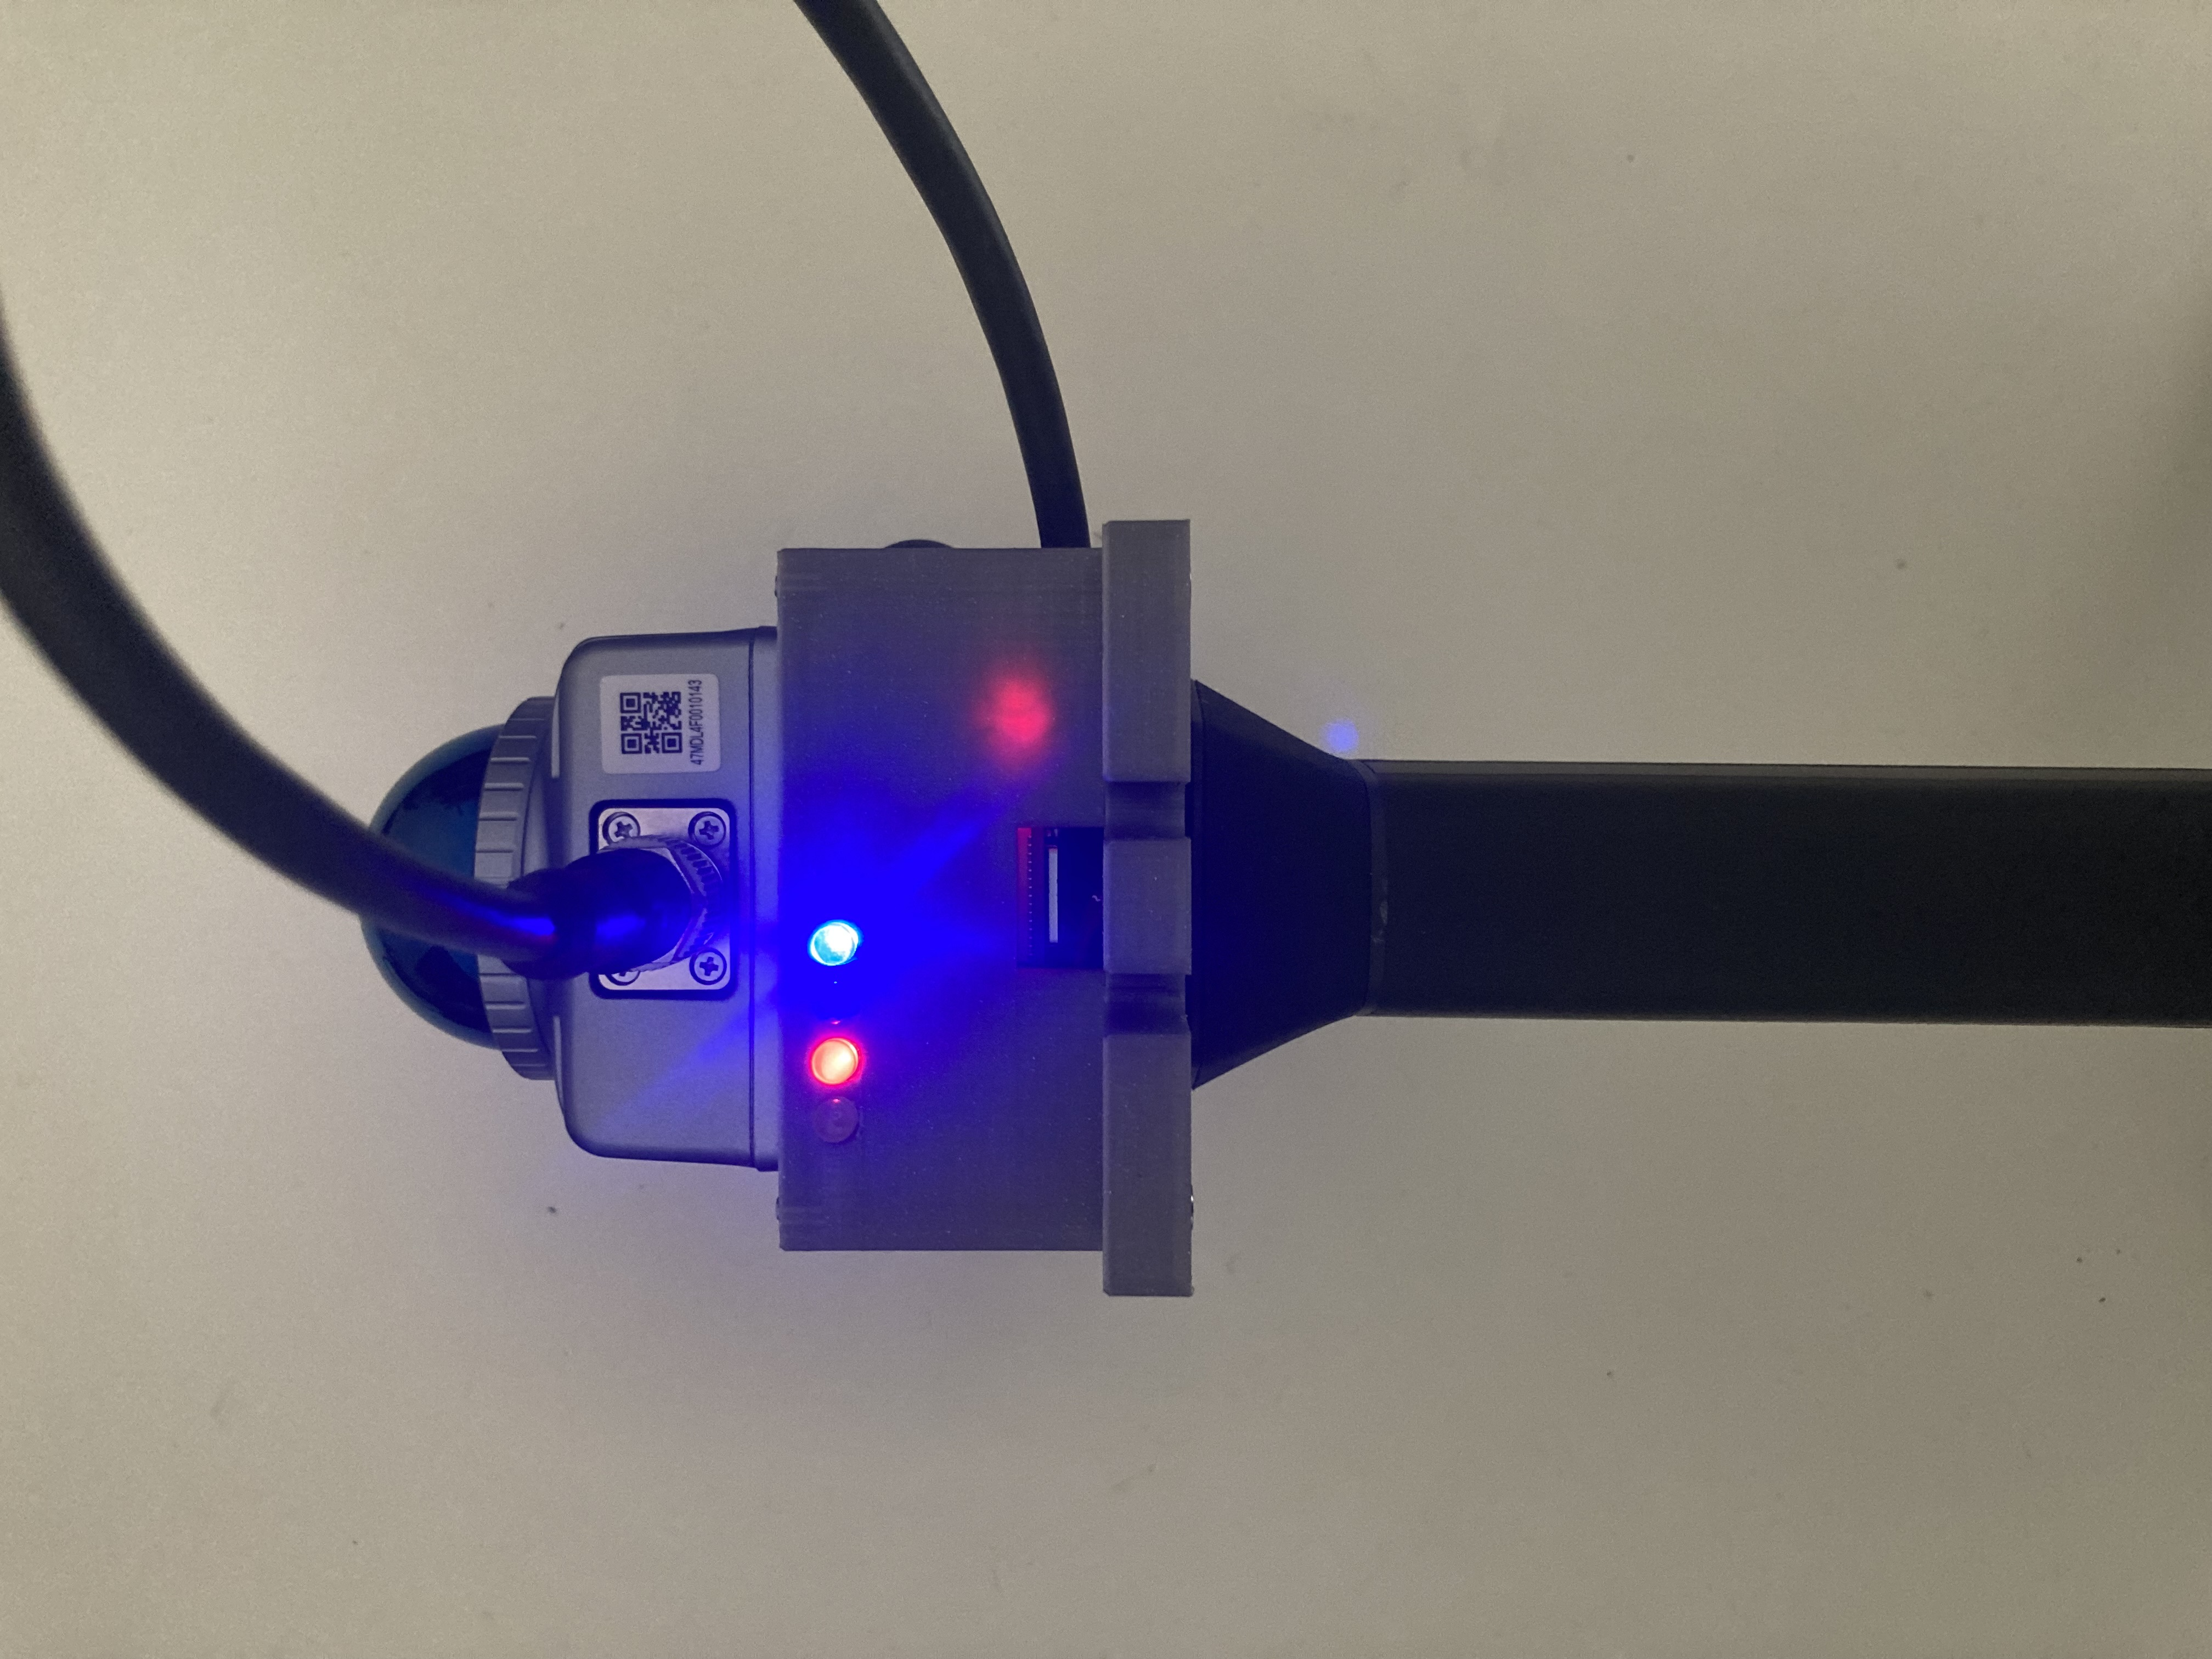
\includegraphics[width=\textwidth, angle = -90]{IMG_95011.jpg}
		\caption{MANDEYE DEV "no USB drive" error - blinking red light.}
		\label{fig:m18}
	\end{subfigure}
	\hfill
	\begin{subfigure}[b]{0.45\textwidth}
		\centering
		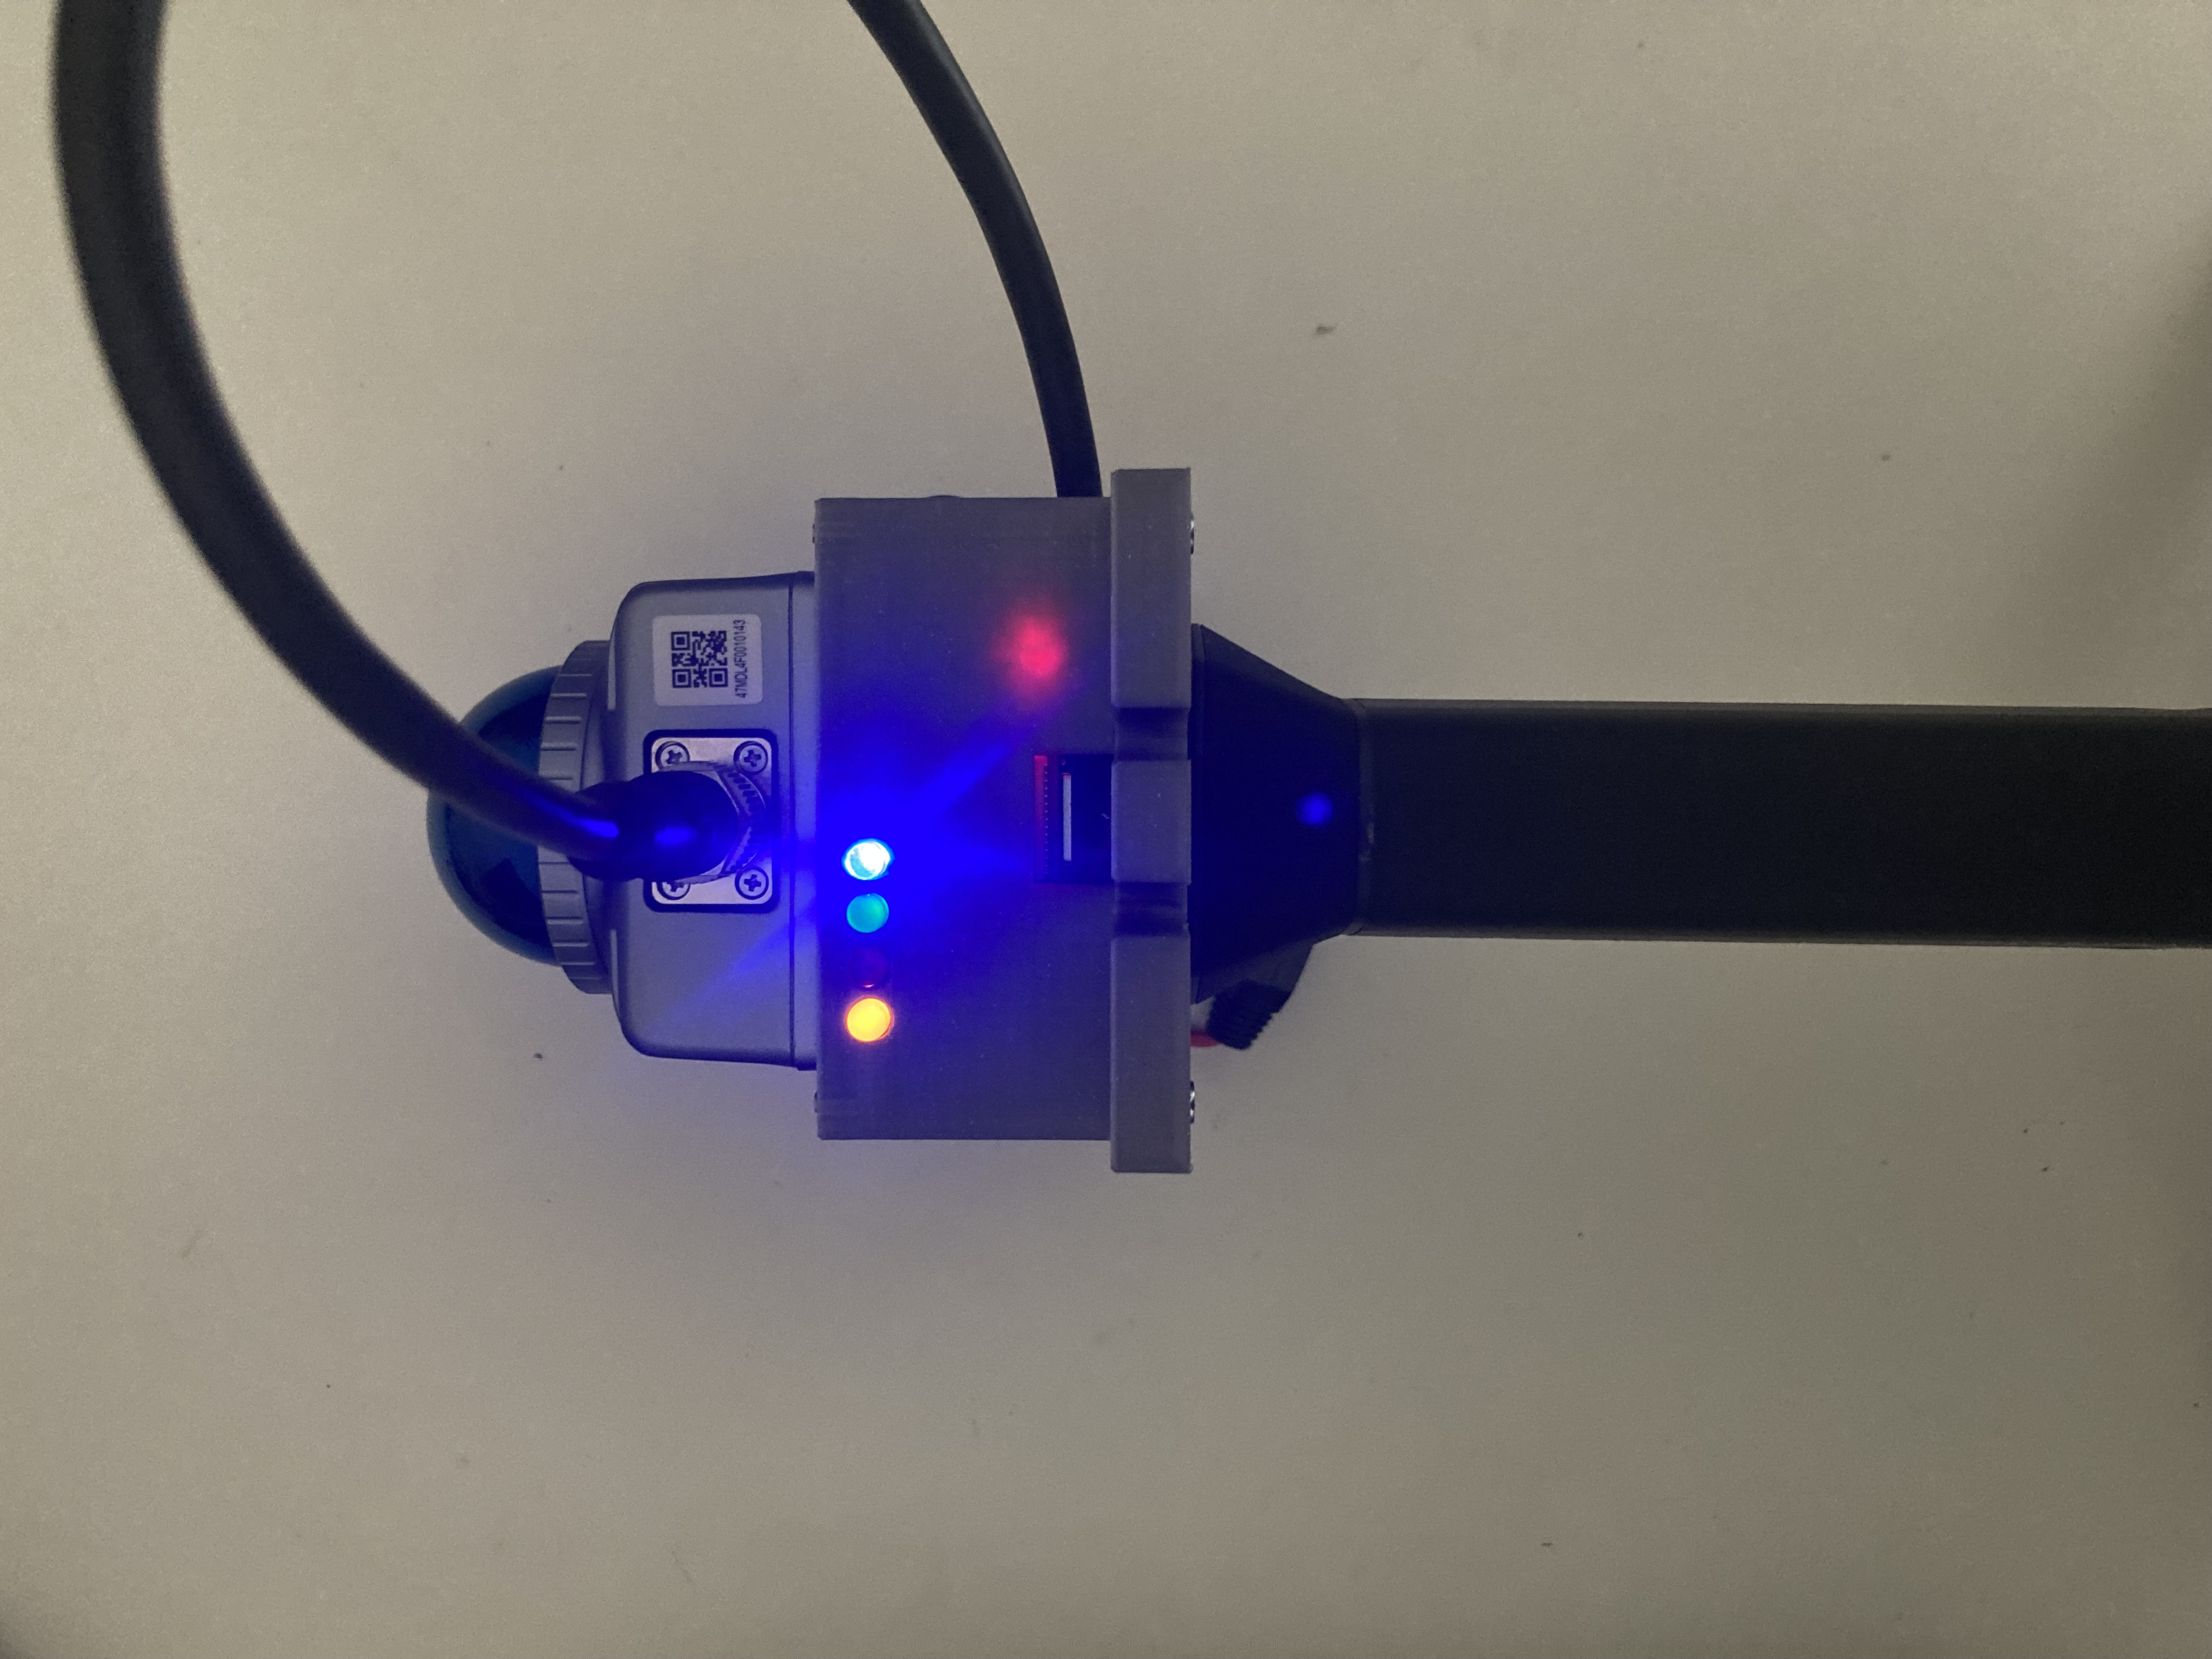
\includegraphics[width=\textwidth, angle = -90]{IMG_95021.jpg}
		\caption{MANDEYE DEV "no communication with LiDAR" error - blinking yellow and green lights.}
		\label{fig:m28}
	\end{subfigure}
	\caption{MANDEYE DEV error indicators.}
	\label{fig:mandeye_harware5}
\end{figure}
